\documentclass{sig-alternate}

\usepackage{amsmath}
\usepackage[linesnumbered,boxed]{algorithm2e}
\usepackage{subfigure}
\usepackage{epstopdf}
\usepackage{graphicx}
\usepackage{color}
\usepackage{multirow}
\usepackage{colortbl}
\definecolor{mygray}{gray}{.4}

\makeatletter
\def\@copyrightspace{\relax}
\makeatother

\begin{document}
\title{The Spiral of Silence and Its Application in Recommender System}
\numberofauthors{1}
\author{Paper 118}

%\numberofauthors{2}
%\author{
%\alignauthor
%Jie Huang, Dugang Liu, Chen Lin\\
%\affaddr{Department of Computer Science}\\
%\affaddr{Xiamen University}\\
%\affaddr{422 Siming South Road}\\
%\affaddr{Xiamen, Fujian, China, 361005}\\
%\email{chenlin@xmu.edu.cn}
%%4th. auther
%\alignauthor Jian Pei\\
%\affaddr{School of Computing Science}\\
%\affaddr{Simon Frasor University}\\
%\affaddr{8888 University Drive}\\
%\affaddr{Burnaby, BC, Canada, V5A 1S6}\\
%\email{jpei@cs.sfu.ca}
%}
\maketitle
\begin{abstract}
Are people in recommender systems less willing to speak out if they perceive they are in the minority? We testify the famous ``spiral of silence'' theory in actual recommender systems. We find that not only minority opinion holders incline to remain silent, but also the incline is enlarged if the opinion climate gets stronger. Furthermore, we discover that (1) For niche items, people are less likely to express negative opinions and more likely to give positive responses. The tendency is weakend for popular items, thus resulting in a spiral process where the average rating for each item increases given more ratings received, slightly decreases after a certain time point, and finally converges. (2) People assess the ``opinion climate'' in a ``quasi-statistical '' sense, which is highly affected by how they identify themselves to different communities and the opinion leaders. (3) A hardcore group of people, who are more active to reveal minority opinions, exists in every recommender system. In general, the personality of hardcore is related to attitude certainty.  (4) People are more willing to demonstrate dissents for popular items and items that they are interested on. People feel more obligated to praise a criticized item than the opposite, to criticize an appreciated item.  The phenomenon of silent minority harms the performance of conventional recommender systems. We propose novel models which assume that the probability a user willing to express opinion is dependent on the rating and how the rating divergent to the perceived opinion climate. Furthermore, we utilize our empirical discoveries to guide the building of recommender models. We model the formation of community, opinion leaders, hardcore personality and item popularity to enhance recommendation performance.  Experimental results demonstrate that our models  outperform state-of-the-art recommendation models.
\end{abstract}

% A category with the (minimum) three required fields
\category{H.4}{Information Systems Applications}{Miscellaneous}


\terms{Algorithms,Verification}

\keywords{Spiral of Silence, Missing not at Random, Recommender System}

\section{Introduction}\label{sec:introduction}
%The theory

In 1974, German political scientist Elisabeth Noelle-Neumann proposed the Spiral of Silence Theory\footnote{In the remaining of this paper, the Spiral of Silence theory will be referred as ``the theory''.}~\cite{Neolle-Neumann1993spiral}. The theory states that, due to the ``fear of isolation'', people are less willing to express their opinions if they perceive that they are not supported by the majority. It results in a spiral process in which the majority opinion receives growing popularity while other opinions are gradually pushed back. The process continues until the majority opinion ultimately becomes a social norm.

%Related Empirical Study
The theory has been acknowledged as ``one of the most influential recent theories of public opinion formation''~\cite{Kennamer1990Self}. In the literature of mass communication and political science, many studies testified the theory. Typically, they conducted surveys and asked subjects to rate the willingness to speak out (i.e. enter a conversation, vote, donate, etc.) if their opinions are in the minority. However, this type of experiment protocols may be problematic, because the findings are based on hypothetical willingness instead of actual willingness~\cite{Carroll1997Perceived}. The theory in its online form also triggers considerable critiques. Some researchers pointed out that, within the online context, factors such as anomity might decrease the fear of isolation and thus empower ``people in the minority to speak up more''~\cite{mcdevitt2003spiral}.

%Contribution: Empirical Study, discoveries
Our first contribution in this work is to empirically verify the theory in terms of actural willingness to speak out in Recommender Systems (RS). We use several real data sets to analyze response patterns given how the users' opinion diverge from the perceived ``opinion climate''. Our study suggests that, especially in the beginining, negative feedback tend to self-censor,  which triggers an upward spiral of average rating for each item.

We then further examine some key components in the theory  The key components include: (1) The perceptron of ``opinion climate''. The theory asserts that people use their ``quasi-statistical'' sense to assess current majority opinion. Our results reveal that, assessment of ``opinion climate'' might be related to the social group they identify themselves and the opinion leaders. (2) The existence of ``hardcore groups''. The theory presumes that some people are more active while the rest are more reluctant to respond. We empirically verify the existence of a consistent hardcore group. Hardcore users tend to choose more extreme rating values. (3) The strategies to remain silent. The theory presumes that users might choose different strategies to remain silent according to the nature of items. We observe that, for popular items, people are more willing to speak out different opinions. Personal interest also has a significant effect on the response patterns. Users are more prone to praise a criticized item than to criticize an appreciated item.


%Challenge to RS
The phenomenon of ``silent minority'' will harm the performance of RS. Fig.~\ref{fig:example} gives an illustrative example. Suppose user $u_1$ is a sensitive user who only responds to items on which he agrees with the majority. Given his responses, a conventional recommender will estimate his preferences as the average user preference. For example, a collaborative filtering recommender will determine $u_1$'s nearest neighbor as $u_2,u_3$, as the similarities    $s_{1,2}$ between $u_1,u_2$ and $s_{1,3}$ between $u_1,u_3$ are the highest. It leads to a predicted rating $r_{1,1}=\frac{s_{1,2} r_{2,1}+s_{1,3} r_{3,1}}{s_{1,2}+s_{1,3} }=5$ for item $v_1$. As we can see from the example, the prediction is severely biased.

%running example
\begin{figure}\label{fig:example}
\centering
\tiny
\begin{tabular}{|c|c|c|c|c|c|}
\hline
u/v & $v_1$ & $v_2$ & $v_3$ & $v_4$ & $v_5$ \\\hline\hline
 $u_1$ & \color{mygray}2 & 3 & & 3 &  \\\hline
 $u_2$ & 5 & 3 & &  &2 \\\hline
 $u_3$ & 5 & 3 &5 & 3 & \\\hline
 $u_4$ &  &  &2 & 3 & 4 \\\hline
 $u_5$ & 5 &  &2 &  &  1\\\hline
\end{tabular}
\caption{A toy example, ratings in gray are ``hidden'' opinions}
\end{figure}

%Related Work
To address the challenge of ``spiral of silence'', one need to model the missing ratings as missing not at random observations(a.k.a. MNAR). In the RS community,  MNAR models explicitly generate user response by user ratings~\cite{Hernandez-Lobato2014Probabilistic,Steck2010Training,Marlin2009Collaborative}. Instead of optimizing $p(R|\Theta)$, which is the likelihood of ratings, MNAR models optimize $p(R,X|\Theta)$, where $X$ is the set of \textit{response} variables indicating whether a rating is missing. Consequently, MNAR models achieve better performance in predicting both ratings and responses.

%Contribution
In the nutshell, our models fall into the MNAR framework. However, for the best of our knowledge, we are the first to apply ``spiral of silence'' theory in recommender systems and consider the perception of support as a factor in an MNAR model. we model the possibility of user ``speaking out'' as dependent on users' perception of opinion climate.  Our model adjusts the bias of response probability by connecting the rating values and opinion climate, thus improves the performances of traditional MNAR models, which are solely based on rating values.  In the experiments on real data sets, our model achieves best results (NDCG 0.79) compared with other state-of-the-art MNAR models(best NDCG 0.7).

We also utilize the findings in our empirical study to build variant models. We incorporate hidden community, hardcore persona and item specific factors into the model. The comparative performances of model variants support the discoveries about the impact of social identity, hardcore groups and silent strategy on self definition of minority. We believe our study sheds insights into bridging social science and computer engineering.

%paper structure
The paper is organized as follows. In Sec~\ref{sec:related} we briefly introduce the related works. In Sec~\ref{sec:empirical} we present our empirical study on several real data sets. In Sec~\ref{sec:model} we propose several model variants, based on the findings in Sec.~\ref{sec:empirical}. In Sec.~\ref{sec:experiment} we demonstrate and analyze comparative performances of the models. Finally, in Sec.~\ref{conclusion} we conclude our contribution and look into the future work.


\section{Related Work}\label{sec:related}
%recommender systems: collaborative filtering
Recently, recommendation system has attracted a lot of research attentions. In the fruitful literature, matrix factorization~\cite{Koren2009Matrix} techniques have exhibited superior performances in rating predictions and become a standard approach. Probablistic matrix factorization~\cite{salakhutdinov2008probabilistic} implement the idea of matrix factorization from a probabilistic generative perspective. It assumes that each rating is randomly sampled from a Gaussian distribution, whose mean is the product of user preference and item aspects. Opinion leaders and social communities can be included in this framework. For example, a SVD style model~\cite{Liu2011Wisdom} factorizes the rating matrix to most representative users. The social recommender~\cite{Jamali2011Generalized} models how a user's rating is affected by his/her trusted friends in a community.

%MNAR

When data is not missing at random, the probability of generating both observations and missing ratings (thus the ``whole'' data set) is not proportional to the likelihood of observed ratings. Marline et.al presented a piorneer work~\cite{Marlin2009Collaborative} of Missing Not At Random (MNAR) models. It assumes that response is a binary variable, which is generated by a Bernoulli distribution associated with the rating value. Along this line, several successive research works introduce new mechanism to generate responses from ratings. A continous rating is allowed in ~\cite{Ling2012Response} with a step function for the probability of generating responses. Such a soft assignment model is further improved in ~\cite{Yang2015Boosting} with a mini batch algorithm. ~\cite{Kim2014Bayesian} adopts an OR operation over per-item, per-user, per-rating-value parameters. The most complicated model is given by ~\cite{Hernandez-Lobato2014Probabilistic}, which proposes seperate generative process for the complete ratings and the responses, and cover the rating matrix by the response matrix as a mask to form the observations.

Another line is to consider a semi-observed variable ``exposure'', which is related to response. Whether the item is exposed to the user, as well as the potential rating determine the response. A few recent works~\cite{Liang2016Modeling,Gopalan2015Scalable} fall into this category. Instead of directly producing a response based on the hidden rating, an alternative approach is to probabilistically relate responses and ratings. For example, ~\cite{Ohsawa2016Gated} presumes a parameter is involved in both processes of generating ratings and responses. Under the MNAR assumptions, conventional evaluation metrics, such as NDCG may fit better to response bias~\cite{Pradel2012Ranking}. An approximate evaluation metric in top N observations is presented in~\cite{Steck2010Training}.

%dynamics of public opinion
The dynamics of public opinion is a long refreshing research topic. Many empirical studies are performed in various domains. Some researchers have observed the trend of increasing average ratings. They offered several explanations. The first one is selection bias hypothesis. It believes that  users select and rate entities they are likely to like~\cite{Dalvi2013Para}. The second hypothesis is choice-supportive bias~\cite{Cohen1970dissonance}. According to the choice-supportive bias hypothesis, since users take too much efforts in finging a product, they will refuse to admit their poor judgment. The third hypothesis is that more reviews bring in more self-promotion spams~\cite{Jindal2008Opinion}. On the controry, some researchers find that later ratings are on average lower than earlier ratings~\cite{Godes2012Sequential}. The possible explanation is that, the volumn of reviews restrict one's ability to diagnose previous reviews. Therefore when previous reviewers are very different, more reviews may  lead to more purchase errors and lower ratings. Hu et.al observed a J-shaped distribution~\cite{Hu2009Overcoming}, presumably driven by purchasing bias (selecting higher product valuations) and under-reporting bias (report only when it is to ``brag or moan'').

%conclusion
Our empirical study shows that, pure positive ratings ($3,4$ within a range of $[0,5]$ ) are not dominant in recommender systems. The trend of average ratings is not globally monotone. We should also point out that, although the above biases make senses, we believe that our hypothesis in this paper is more reasonable. By introducing the ``opinion climate'', we provide a baseline for judging positive and negative opinions. Our experimental results prove that such a baseline  improves models which consider the polarity of opinions simply by the rating values.



\section{Empirical Study}\label{sec:empirical}
%data sets
We use several real data sets. The first one is Movielens1M, which is a collection of over 1M ratings on movies in the movielens website during a period of ??. The ratings are made on a 5-star scale. More than half of the ratings are positive feedbacks ($4,5$).  The second one is Eachmovie, which include nearly 2.6M ratings on films and videosis over a course of 18-months experiment. The  ratings are in the range of $(0,1)$ . Almost half of them are positive feedbacks ($>0.6$). The two data sets are the most commonly used benchmarks in recommender systems.The ratings come with timestamps, so we can analyze patterns between user responses and current opinion climate. Each item is labeled by at least one tag.

We also use the recent Yahoo! data set, which is a set of ratings on songs through the Yahoo! web-scope data sharing program. The data set contains two subsets of ratings. The first (Yahoo!user) set consists of ratings supplied by users during normal interaction with Yahoo! Music services. The second source consists of ratings collected during an online survey, when each of the first 5400 users in Yahoo!user set was asked to provide exactly ten ratings for randomly selected songs. The ratings in Yahoo! dataset do not come with timestamps.

The Yahoo! data sets provide unique opportunities to testify the spiral of silence theory.  The random setting corresponds to a scenario where users are forced to response, against his actual willings. The user selected setting corresponds to a scenario where users are free to hide their responses. Therefore we can compare user's behaviors within different restrictions to study the key components of the theory.
\begin{table*}[htbp]
\centering
\caption{Statistics of the data sets}\label{tab:statistics}
\begin{tabular}{|c|c|c|c|c|c|c|c|}
\hline
Dataset &\#users & \#Items & \#Ratings & Negative & Positive  & Time & \#Tags\\\hline\hline
Movielens & 6,040 & 3706 & 1,000,209 & $57.52\%$ &$42.48\%$ & 34 months&18 \\\hline
Eachmovie & 61,131 & 1,622 & 2,559,107 & $54.72\%$ & $45.28\%$ &18 months &10 \\\hline
Yahoo!user & 15,400 & 1000 & 311,704 & $40.13\%$ & $59.87\%$ & N/A & 0\\\hline
Yahoo!random & 5400 &  1000 & 54,000 & $8.79\%$& $91.21\%$ &N/A & 0\\
\hline
\end{tabular}
\end{table*}

\subsection{Silent Minority}
%Do response patterns differ in response to opinion divergence?
 We use the common RS data sets to investigate the silent minority. We first show the historgram of ratings in each data set in Fig.~\ref{fig:histe} and Fig.~\ref{fig:histm} respectully. For each rating, we compute its difference to the current average ratings on the item. The rating divergence is defined as $d=r_{i,j,t}-\hat{r_{j,t}}$, where $r_{i,j,t}$ is the rating by user $i$ on item $j$ at timestamp $t$, and $\hat{r_{j,t}}$ is the average rating on item $j$ by timestamp $t$. We report the distribution of $d$ in three different time segments in Fig.~\ref{fig:de} and Fig.~\ref{fig:dm}. The \textit{first}(green curve) distribution is based on the 95th and 100th ratings received for each item v.s. the average of first 95 ratings on the item. The \textit{end}(red curve) distribution is based on the last 5 ratings received for each item v.s. the average of all ratings on the item. For the \textit{middle} distribution, we chronologically divide the ratings for each item into two parts, and the computation is excecuted on the last 5 ratings on the first devision.  We also report a ``background'' distribution of $\bar{d}=r_{i,j,t}-\hat{r_{j}}$, where $\hat{r_{j}}$ is the average rating on item $j$ at all times.
\begin{figure}[htbp]
\centering
\subfigure[$r$ in Eachmovie]{
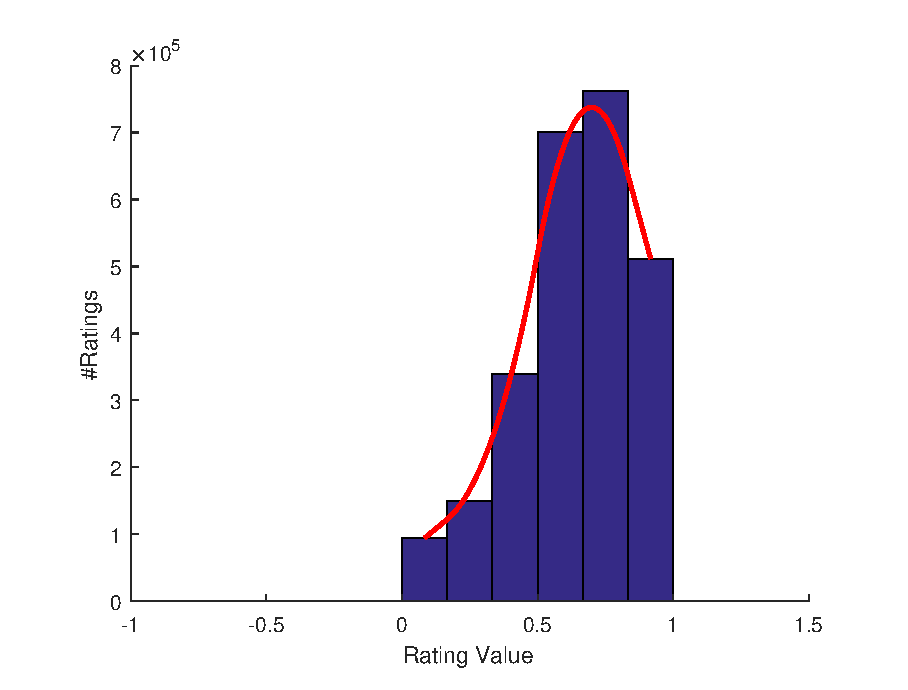
\includegraphics[width=0.2\textwidth]{fig2_eachmovie_hist.eps}\label{fig:histe}}
\subfigure[$d$ in Eachmovie ]
{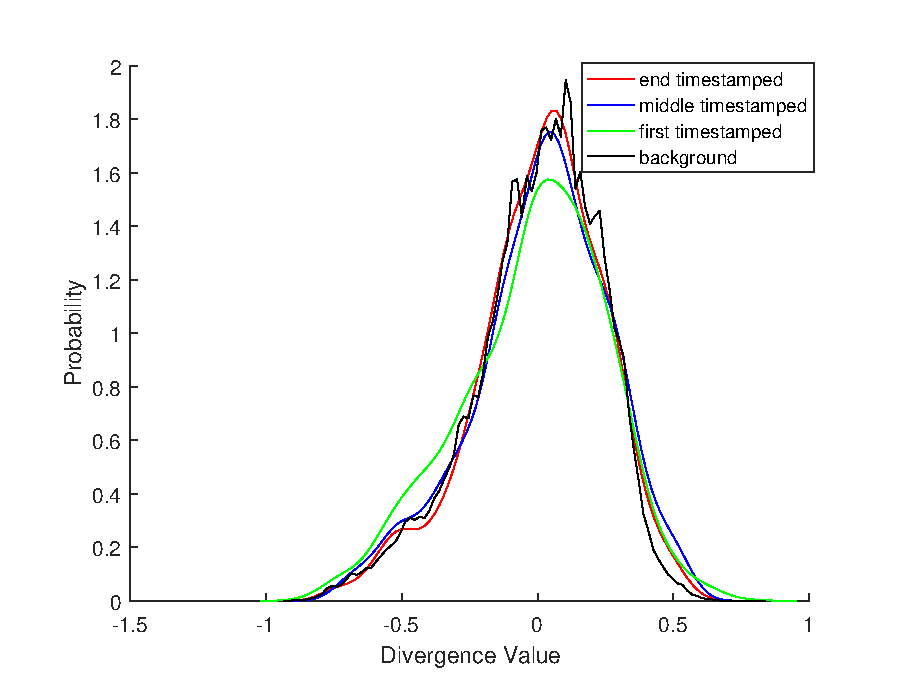
\includegraphics[width=0.2\textwidth]{fig2_eachmovie_npopular.eps}\label{fig:de}}
\subfigure[$r$ in Movielens]{
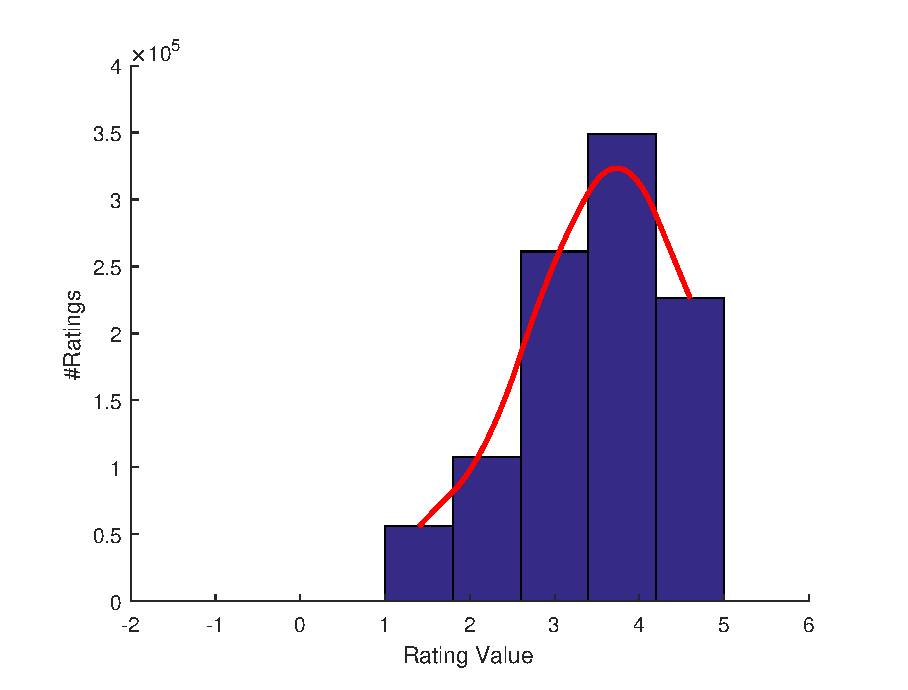
\includegraphics[width=0.2\textwidth]{fig2_movielens_hist.eps}\label{fig:histm}}
\subfigure[$d$ in Movielens]
{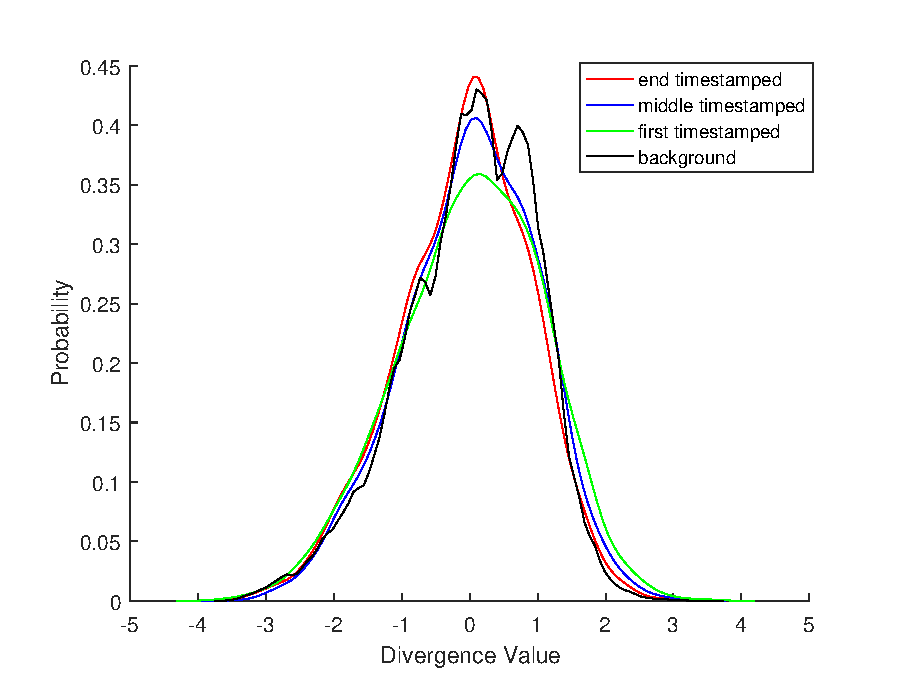
\includegraphics[width=0.2\textwidth]{fig2_movielens1M_npopular.eps}\label{fig:dm}}
\caption{Distributions of rating value $r$ and rating divergence $d$}\label{fig:minority}
\end{figure}


We have the following observations in both the data sets. (1) The majority ($>75\%$) of rating divergence falls in the small range of $[-1,1]$ (in Eachmovie $[-0.2,0.2]$). Minority opinion holders have a strong tendency to keep silent. (2) All distributions are lft skewed. The mass of distribution of rating divergence locates at the right of origin. (3) The timestamped distributions offer us a better opportunity to analyze the response patterns, as they are smoother and single peaked. We can see that as time goes by, the curves are becoming shallower and moving to the left. This suggests that, when the opinion climate is stronger (with more supporters), minority opinion holders are less likely to speak out. It also suggests that when the target item is not popular, people are less likely to give negative feedback and more likely to give positive feedback. We will look into this issue in the next subsections.

\begin{figure}[htbp]
\centering
\centering
\subfigure[Eachmovie]{
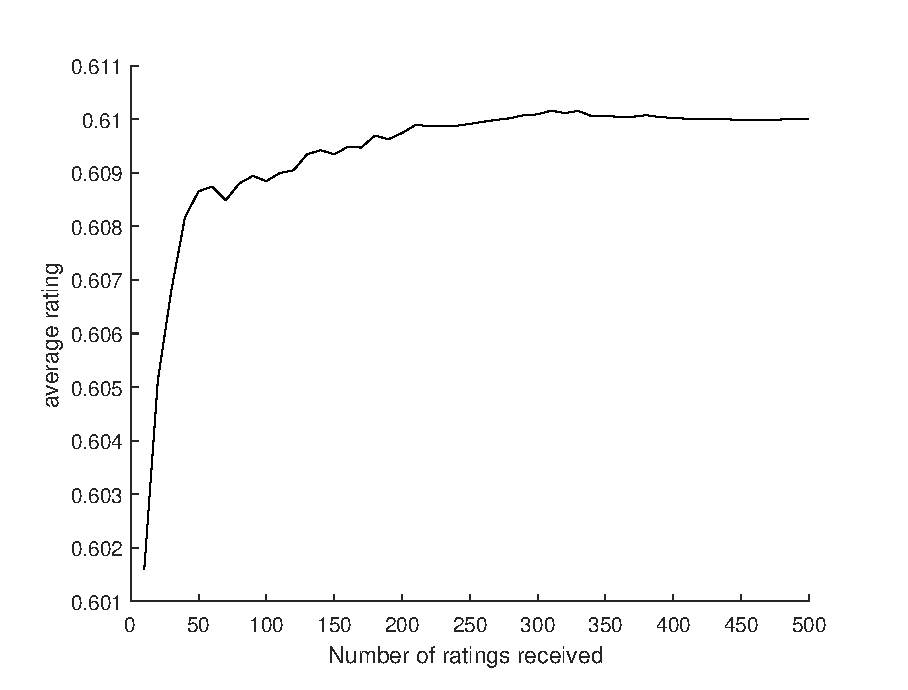
\includegraphics[width=0.2\textwidth]{fig3_eachmovie_npopular.eps}
}
\subfigure[Movielens]{
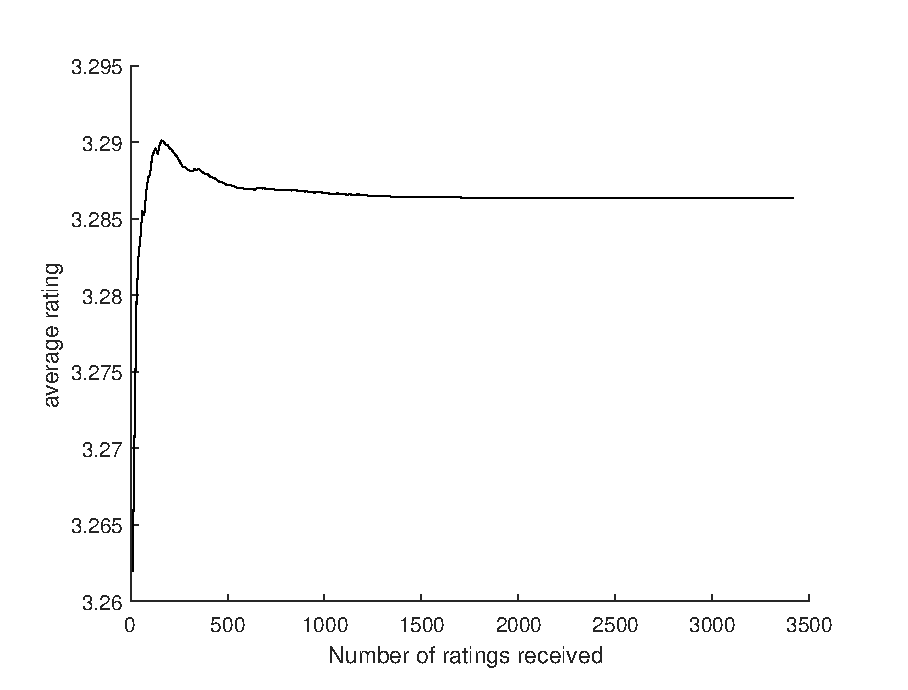
\includegraphics[width=0.2\textwidth]{fig3_movielens1M.eps}
}
\caption{The spiral of average rating v.s. the number of ratings received}\label{fig:spiral}
\end{figure}

When users refuse to speak out relatively negative opinions, more positive feedback is observed while negative feedback is infrequently voiced. In theory this will lead to enlarging average rating. We plot the average rating for each item when they have $x=10\times k$ ratings, $k=1,\cdots,50$ for Eachmovie and $k=1,\cdots,350$ for Movielens. As shown in Fig.~\ref{fig:spiral}, two discoveries are clear. (1) An upward spiral is indeed activated. With more ratings received, the average rating for each item  increases. (2) In the tail (approximately more than $350$ ratings in Eachmovie and $500$ in Movielens), the average rating begins to decrease. This trend suggests that for popular items, the people are more incline to give negative feedback.

We have shown that the silent minority, defined as the group of users who hold different ratings $d>\frac{\max(r)-\min(r)}{5}$, is universally observed in many recommender systems. For the yahoo! data set, there is no information about when the ratings are recorded. However, from the comparison between the random subset and user selected subset in Fig.~\ref{fig:yahoo}, we see that, when users are not forced to express their opinions, the distribution is much wider, with multiple peaks at a large scale of $[-2,2]$. Furthermore, they produce significantly less negative feedback and much more positive feedback. Thus our discovery of spiral of silent negative feedback in the common recommender systems is again verified.

\begin{figure}[htbp]
\centering
\centering
\subfigure[Yahoo!random]{
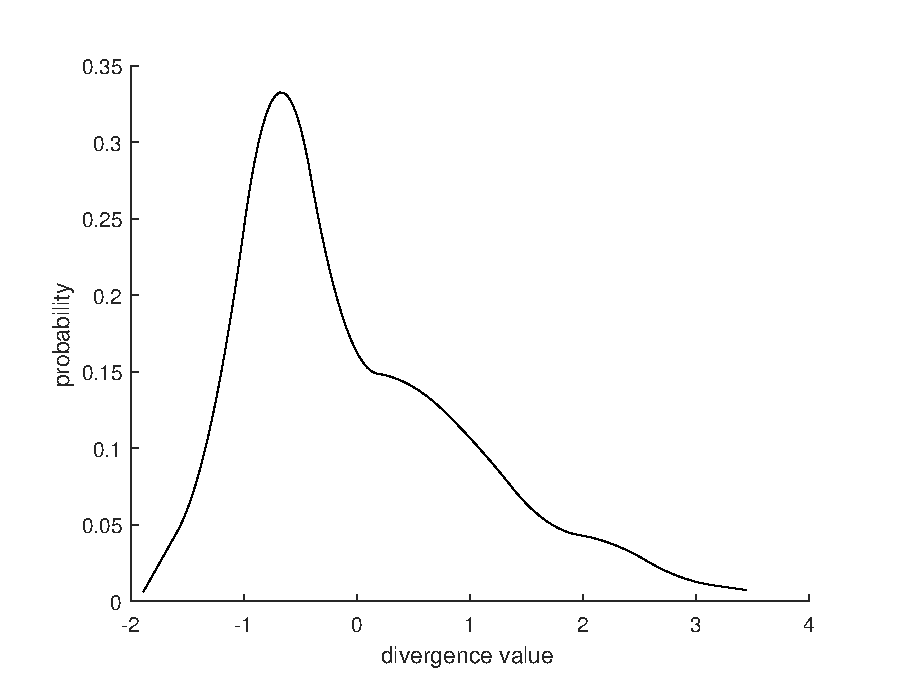
\includegraphics[width=0.2\textwidth]{fig4_random.eps}
}
\subfigure[Yahoo!user]{
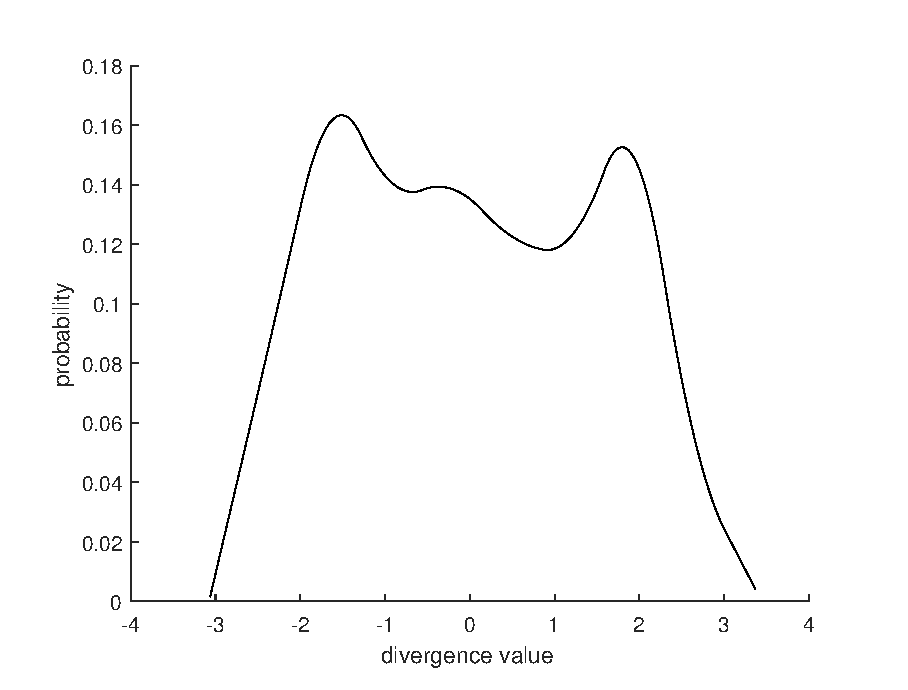
\includegraphics[width=0.2\textwidth]{fig4_user.eps}
}
\caption{The comparative probability distribution of rating divergence in Yahoo!}\label{fig:yahoo}
\end{figure}

\subsection{Opinion Climate}
Opinion climate is a coined term to describe the mainstream opinion. For a thorough understanding of how the opinion climate develops and influences response patterns, we conduct the following studies on the Yahoo! data set.
%the information is overwhelming
In the theory, opinion climate is highly affected by the mass media. In recommender systems, opinion leaders play a similar role as mass media. We select $10$ most active users $O$ (with largest number of ratings) as opinion leaders, and compute the average rating within opinion leaders $\hat{r_j}=\frac{\Sigma_{i\in O}r_{i,j}}{|O|}$. From Fig.~\ref{fig:leader}, we see that, in the random setting, rating divergence to opinion leaders distribute as a normal distribution, while in the user selected setting, distribution of rating divergence to opinion leaders move to the right. The difference between two settings is more obvious than divergence to average people. It shows that opinion leaders magnify users' willingness to remain silence when they hold negative feedback and speak out positive opinions.

\begin{figure}[htbp]
\centering
\centering
\subfigure[Yahoo!random]{
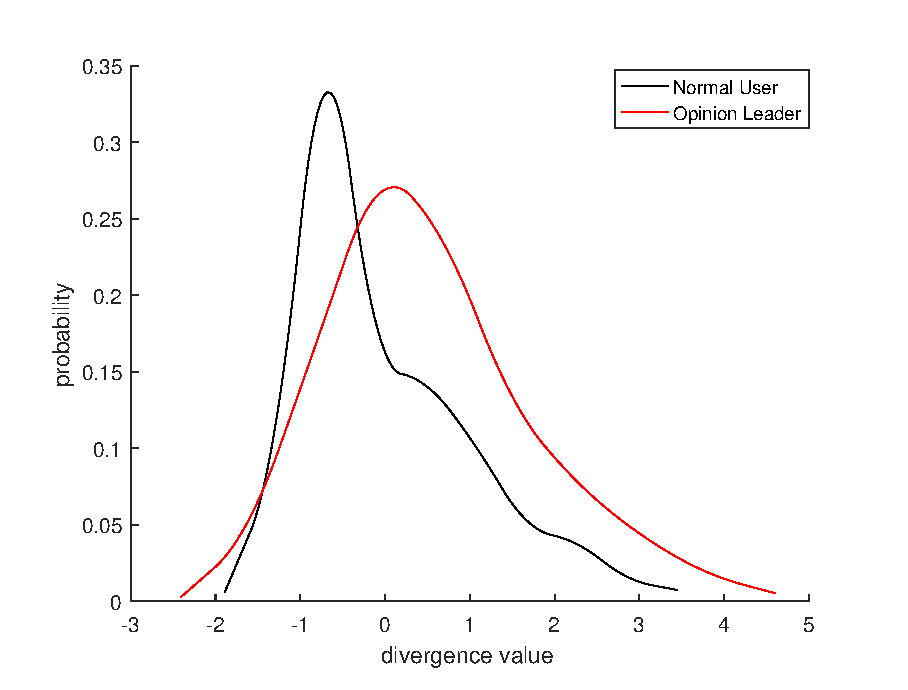
\includegraphics[width=0.2\textwidth]{fig5_random.eps}}
\subfigure[Yahoo!user]{
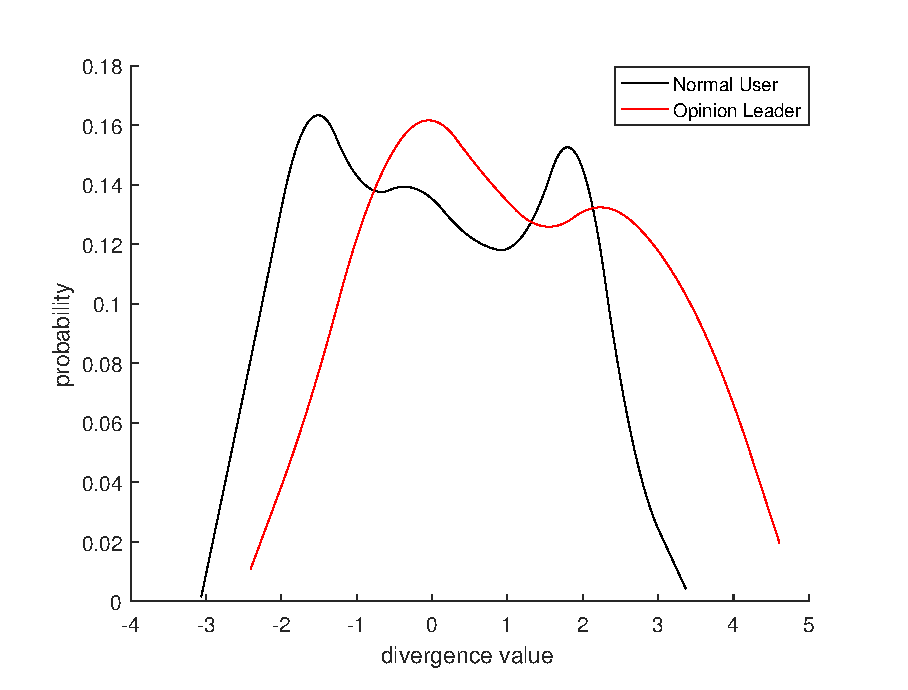
\includegraphics[width=0.2\textwidth]{fig5_user.eps}}
\caption{The comparative distribution of rating divergence to opinion leaders in Yahoo!}\label{fig:leader}
\end{figure}

On the Internet, with the infinite flow of information, users tend to have a limited vision of how others think and behave. They might focus on the opinions alike theirs, and thus perceive a so called ``looking-glass perceptron'' of opinion climate. To study whether the opinion climate is dependent on user communities, we first represent each user as an $M-$dimensional rating vector on the item universe with $M$ items, and proceed to form a cluster $c$ for users by selecting the KNN ($K=50$) users with similar tasts.  We then compute the average of community ratings $\hat{r_{j,c}}=\frac{\Sigma_{i\in c}r_{i,j}}{|c|}$ for community $c$. For each user $u_i$ in community $c$, the rating divergence is   $d=r_{i,j}-\hat{r_{j,c}}$.

\begin{figure}[htbp]
\centering
\centering
\subfigure[Yahoo!random]{
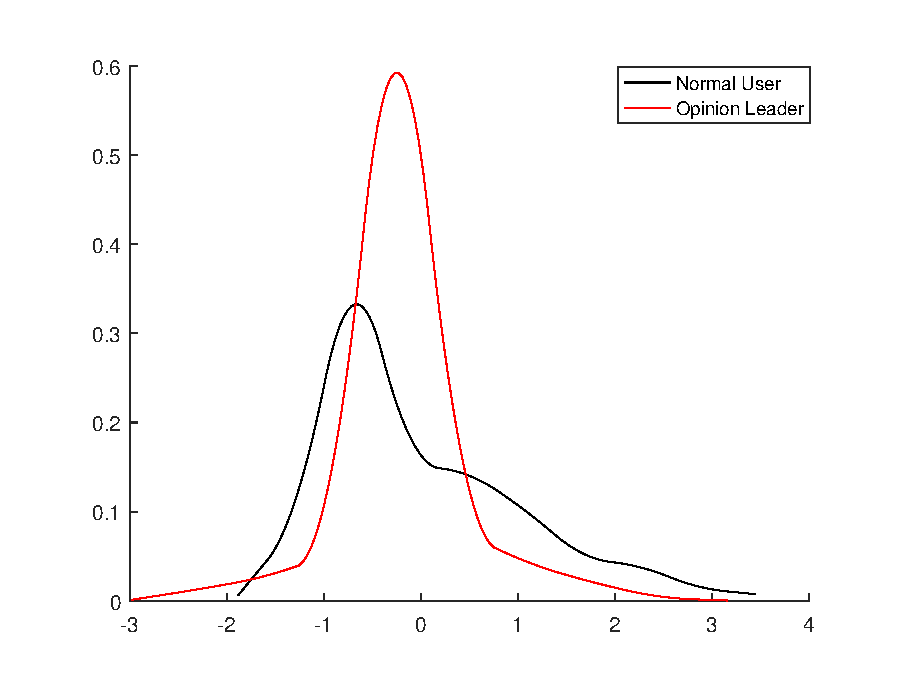
\includegraphics[width=0.2\textwidth]{fig6_random.eps}\label{fig:communityrandom}
}
\subfigure[Yahoo!user]{
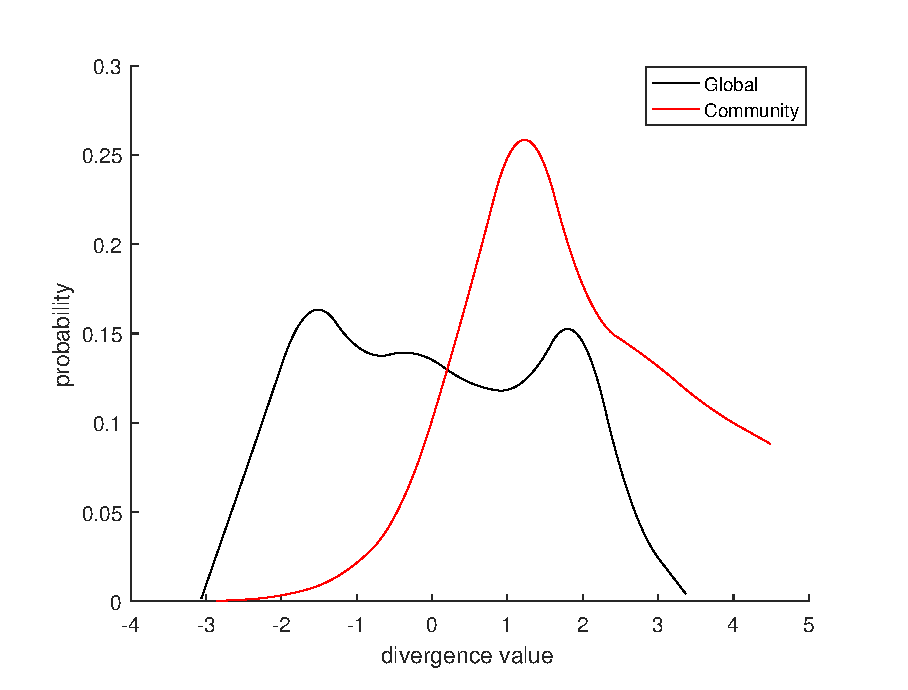
\includegraphics[width=0.2\textwidth]{fig6_user.eps}\label{fig:communityuser}
}
\caption{The comparative  distribution of community specific rating divergence in Yahoo!}\label{fig:community}
\end{figure}

As shown in Fig.~\ref{fig:community}, we have the following observations. (1)In the random setting, rating divergence to community specific majority rating follows a shallow normal distribution, which centers at around $0$.  (2) In the user selected setting, distribution of rating divergence to community specific majority rating is asymmetric. The probability peak is at around $1.25$. For negative opinions, the probability decreases as the divergence increases. For positive opinions, the probability increases as the divergence increases. For extreme positive opinions (at least $1.25$ higher than community specific average rating), the probability decreases as the divergence increases. However, the probability is still larger than negative opinions with equal absolute divergence. These observations strongly indicate that users' perceived opinion climate is actually community specific opinion climate.

\subsection{Hardcore Users}

In the theory, hardcore group is a bunch of people who are brave and willing to express different opinions. We define a ``hardcore'' score for each user, which is $h=\frac{n^h_i}{n_i}$, where $n_i$ is the number of ratings a user $i$ gives to all items, $n^h_i$ is the number of high divergent ratings of user $i$. In Eachmovie, $n^h_i=|N^h_i|$,where $N^h_i=\{|r_{i,j}-\hat{r_{j}}|>0.3\}$. In Movielens, $n^h_i=|N^h_i|$,where $N^h_i=\{|r_{i,j}-\hat{r_{j}}|>1.5\}$.   We observe a small amount of hardcore users in all data sets. As shown in Tab.~\ref{tab:hardcore}, the size of group reasonably decreases as the threshold of hardcore score increases.

\begin{table}[htbp]
\centering
\caption{Percentage of hardcore groups}\label{tab:hardcore}
\centering
\begin{tabular}{|c|c|c|c|c|}
\hline
Dataset & $h=0.5$ & $h=0.6$ & $h=0.7$ & $h=0.8$ \\\hline\hline
Movielens & 0.006	 & 0.0026 &	0.00099 &	0.0005 \\\hline
Eachmovie & 0.0674 &	0.03174 &	0.01693 &	0.01219\\\hline
Yahoo!random & 0.1672& 0.0885& 0.0470& 0.0230\\\hline
Yahoo!user & 0.4234 &0.2744 & 0.1668 & 0.0884\\\hline
\end{tabular}
\end{table}

We first detect hardcore users in the yahoo data sets, and compare the hardcore users in two subsets. We report the overlap percentage $p_h=\frac{|G_{h}^{random}\bigcap G_{h}^{user}|}{|G_{h}^{random}\bigcup G_{h}^{user}|}$ in Tab.~\ref{tab:overlap}, where $G_{h}^{random},G_{h}^{user}$ are the set of hardcore users with hardcore score $h$ in the random subset and the user selected subset respectfully. We also provide the overlap percentage in theory given that users are uniformly sampled by the probability distribution of hardcore shown in Tab.~\ref{tab:hardcore}. We find that hardcore is a consistent personality of users. Despite of the threshold of hardcore score, the overlap percentage of hardcore users is significantly larger than the theoretical overlap, implying that users do not randomly decide to act hardcore.

\begin{table}[htbp]
\centering
\caption{Percentage of hardcore group overlap}\label{tab:overlap}
\centering
\begin{tabular}{|c|c|c|c|c|}
\hline
 Threshold & $h\geq 0.5$ & $h\geq 0.6$ & $h \geq 0.7$ & $h\geq 0.8$ \\\hline\hline
Actural Overlap& 0.16377 &	0.11737 &	0.0908 & 0.07194 \\\hline
Theretical Overalap & 0.1169 &  0.0658 &  0.0341 & 0.0156\\
\hline
\end{tabular}
\end{table}

It is natural to relate hardcore with attitude certainty, while attitude certainty is represented by an extreme rating value. We then set $h\geq 0.5$ and plot the ratio of extreme ratings versus non-extreme ratings for hardcore and non-hardcore users in all data sets. Extreme ratings are $0,5$ ratings in Movielens and Yahoo! and $0,1$ ratings in Eachmovie. We can see from Fig.~\ref{fig:hardcore} that in three data sets, hardcore users have a higher median ratio of extreme ratings, and the tail is much longer. We also notice that when users are forced to express (the Yahoo!random set), the situation is reversed, hardcore users have a lower median ratio of extreme ratings and a short tail.  This observation is again a supplementary evidence of the clear pattern that hardcore users are more likely to give extreme ratings.

\begin{figure}[htbp]
\centering
\centering
\subfigure[Eachmovie]{
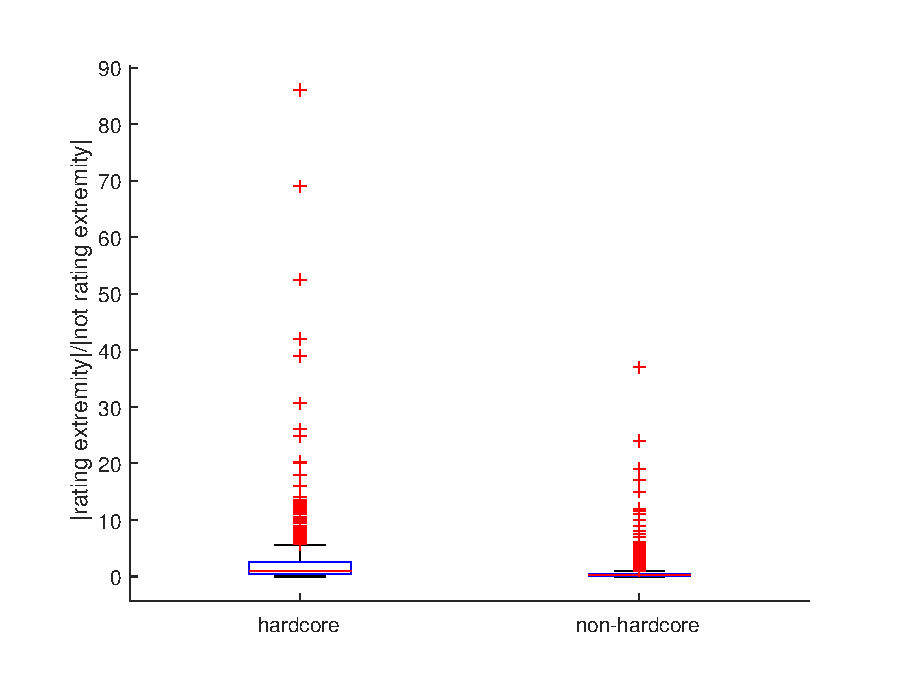
\includegraphics[width=0.2\textwidth]{fig7_eachmovie.eps}
}
\subfigure[Movielens]{
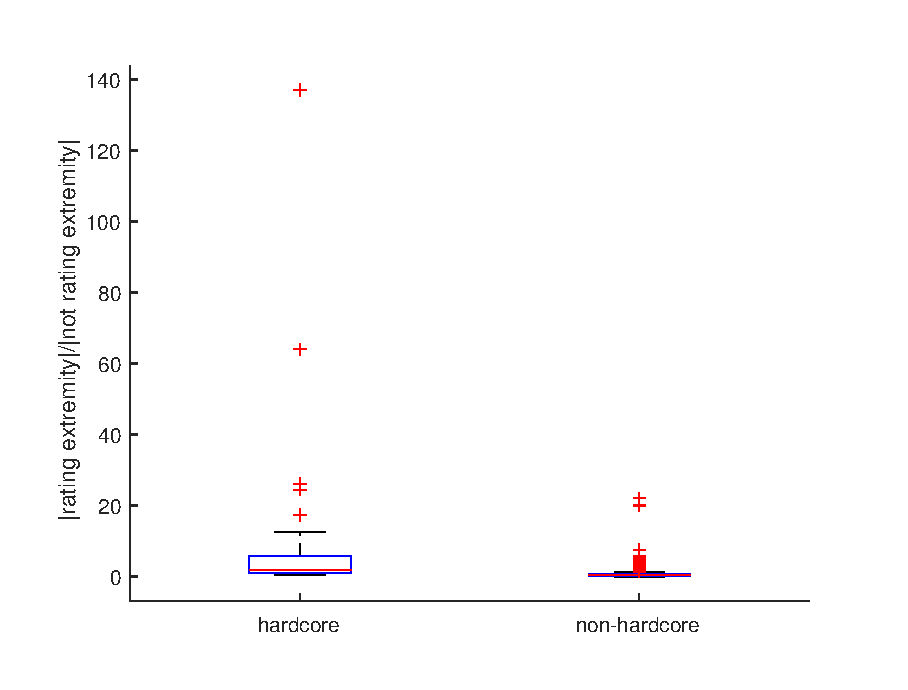
\includegraphics[width=0.2\textwidth]{fig7_movielens1M.eps}
}
\subfigure[Yahoo!random]{
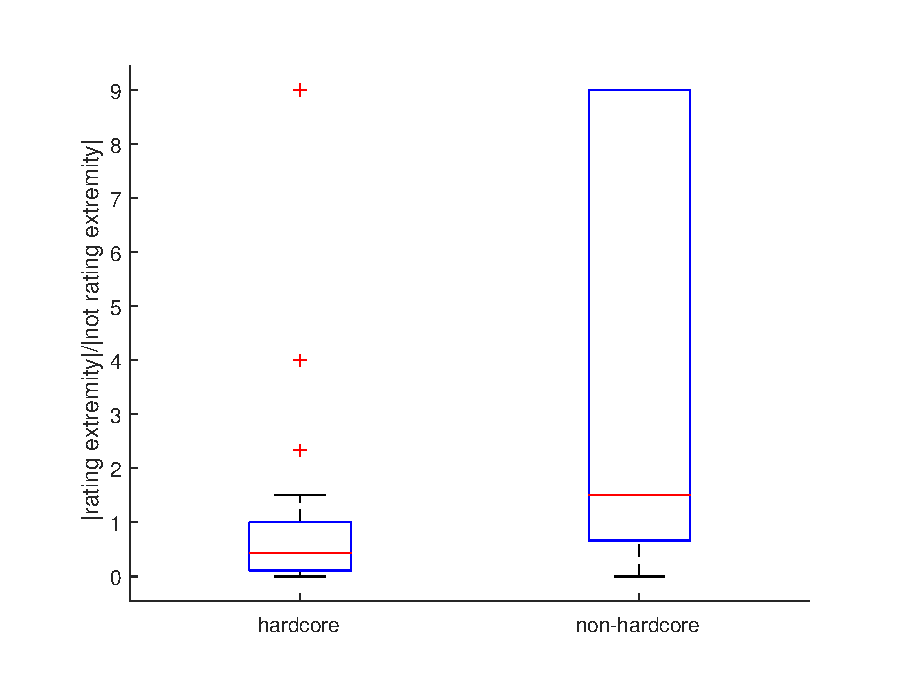
\includegraphics[width=0.2\textwidth]{fig7_random.eps}
}
\subfigure[Yahoo!user]{
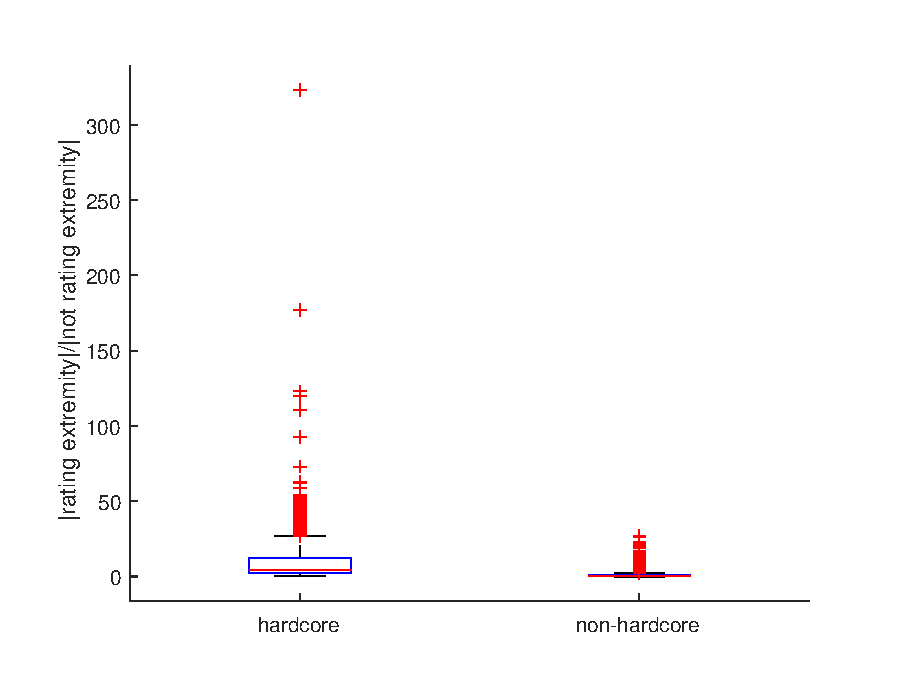
\includegraphics[width=0.2\textwidth]{fig7_user.eps}
}
\caption{Ratio of extreme ratings in hardcore and normal users}
\label{fig:hardcore}
\end{figure}

\subsection{Hardcore and Items}
Finally we study whether the strategies of holding back are dependent on the items. We have already seen the temporal changes in average ratings in common RS data sets in Fig.~\ref{fig:spiral}. In Movielens, the average rating first increases then decreases until converges. There is a similar trend in Eachmovie, although the downward incline is not steep in the tail. One possible reason is that some items are already popular before the Eachmovie project launches and starts to collect ratings. For a thorough study, we present in Fig.~\ref{fig:ratingpopulareachmovie} the average ratings for popular items, which are items that receive more than 500 ratings. We see that for popular items, as the item receives more ratings, the average rating decreases.

\begin{figure}[htbp]
\centering
\begin{center}
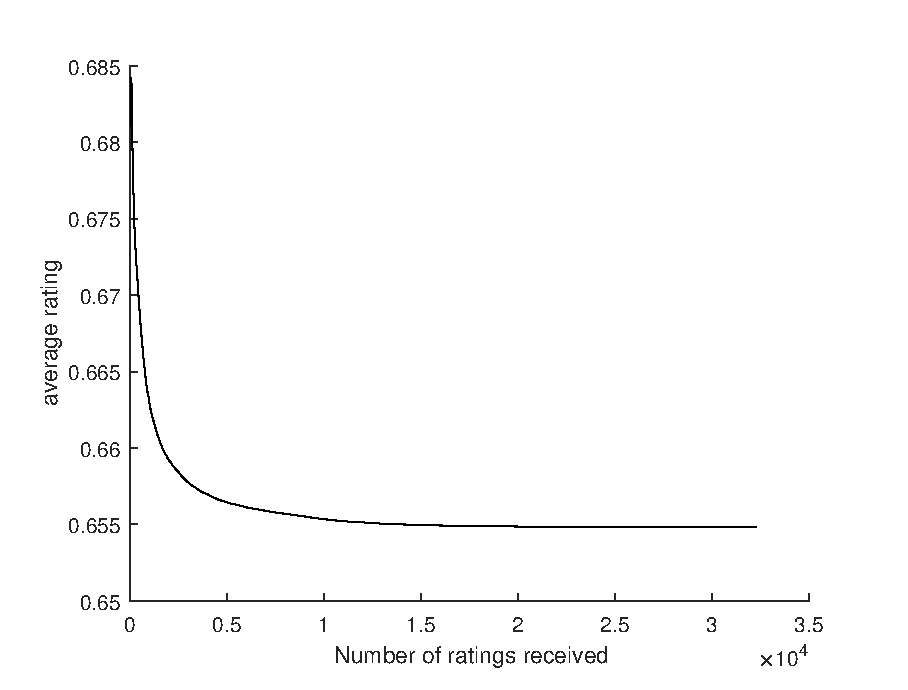
\includegraphics[width=0.2\textwidth]{fig8_eachmovie_popular.eps}
\caption{{Average ratings of popular items in Eachmovie}}
\label{fig:ratingpopulareachmovie}
\end{center}
\end{figure}

Next we study whether the responding is directly related to the popularity of items in Yahoo! data sets. We order the items in the Yahoo! data sets, according to the number of ratings assigned to them. A box plot is shown in Fig.~\ref{fig:popularity} to reveal the distribution of rating divergence versus the order position of popularity. We can see that, in the random subset, the scales of rating divergence are almost the same for popular and unpopular items. In the user selected subset, the scale of rating divergence narrows as the item becomes less popular. It shows that users adopt different strategies for popular items and unpopular items. When users are  not restricted,  they tend to speak out extreme opinions for popular items.

\begin{figure}[htbp]
\centering
\centering
\subfigure[Yahoo!random]{
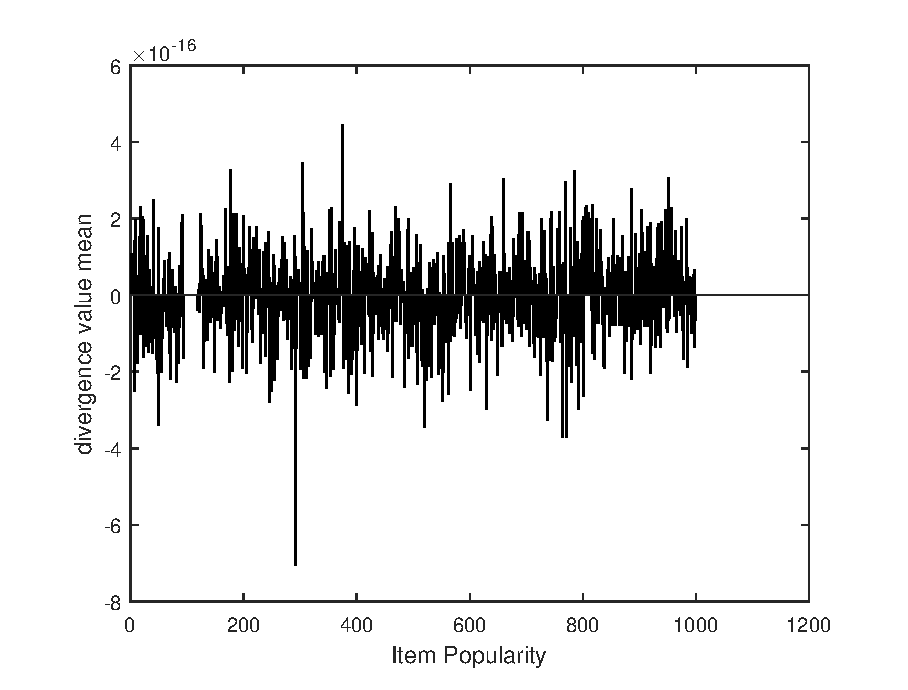
\includegraphics[width=0.2\textwidth]{fig9_random.eps}
}
\subfigure[Yahoo!user]{
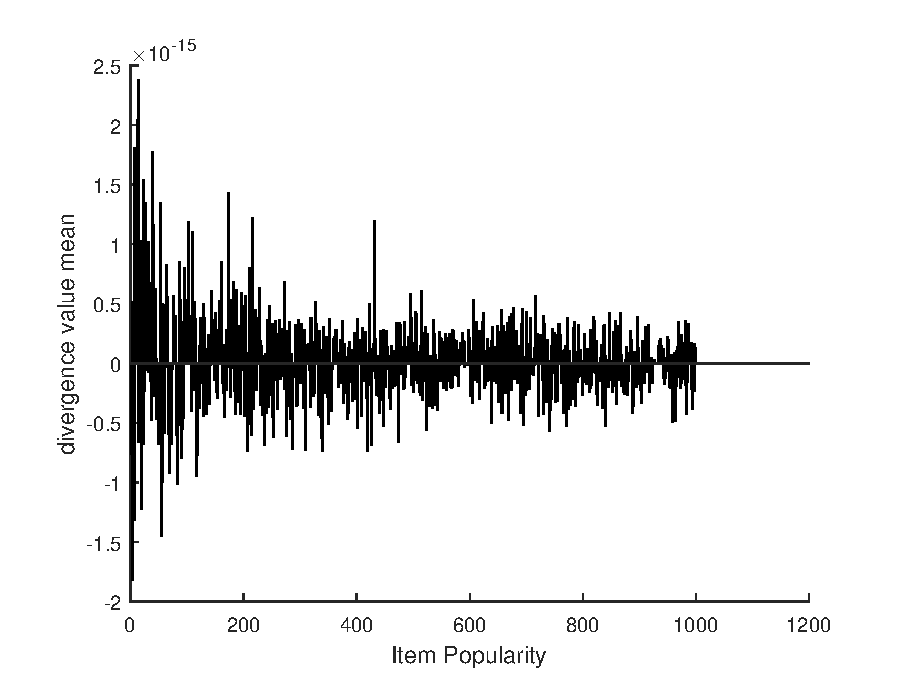
\includegraphics[width=0.2\textwidth]{fig9_user.eps}
}
\caption{The distribution of rating divergence upon item popularity}
\label{fig:popularity}
\end{figure}

It is mentioned in the theory\cite{Neolle-Neumann1993spiral} that hardcore is related to personal interest or importance. To testify this assumption, we select the most rated tag and least rated tag (in number of ratings) for each user, and compute the hardcore score, where $n_i$ is the number of ratings a user $i$ gives to all items associated with the tag.  As shown in Fig.~\ref{fig:personalinterest}, in both data sets, users are more willing to express different opinions (with a higher hardcore score) for most interesting items.

\begin{figure}[htbp]
\centering
\centering
\subfigure[Movielens]{
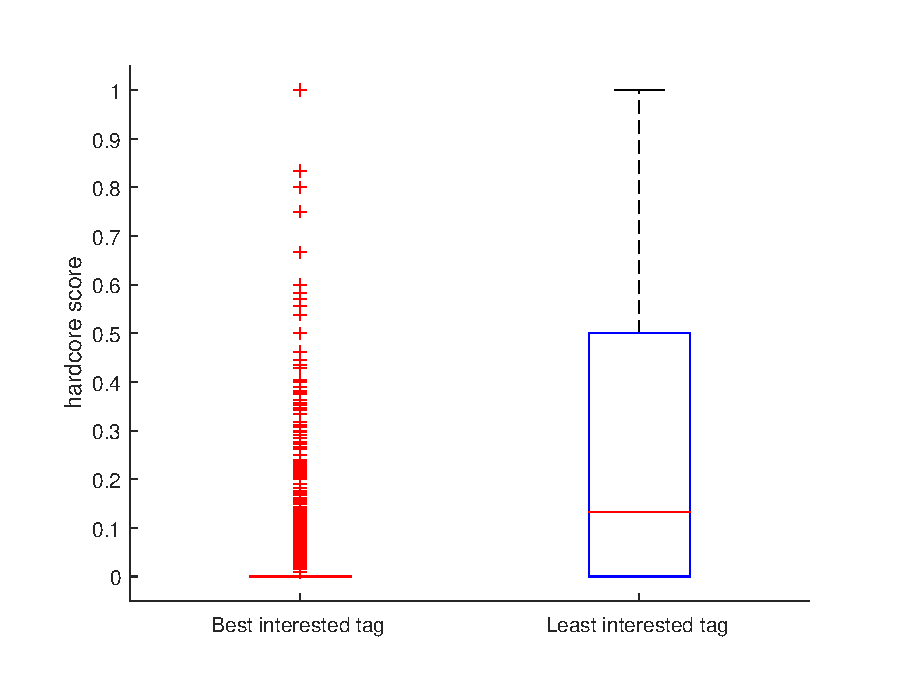
\includegraphics[width=0.2\textwidth]{fig10_movielens1M.eps}
}
\subfigure[Eachmovie]{
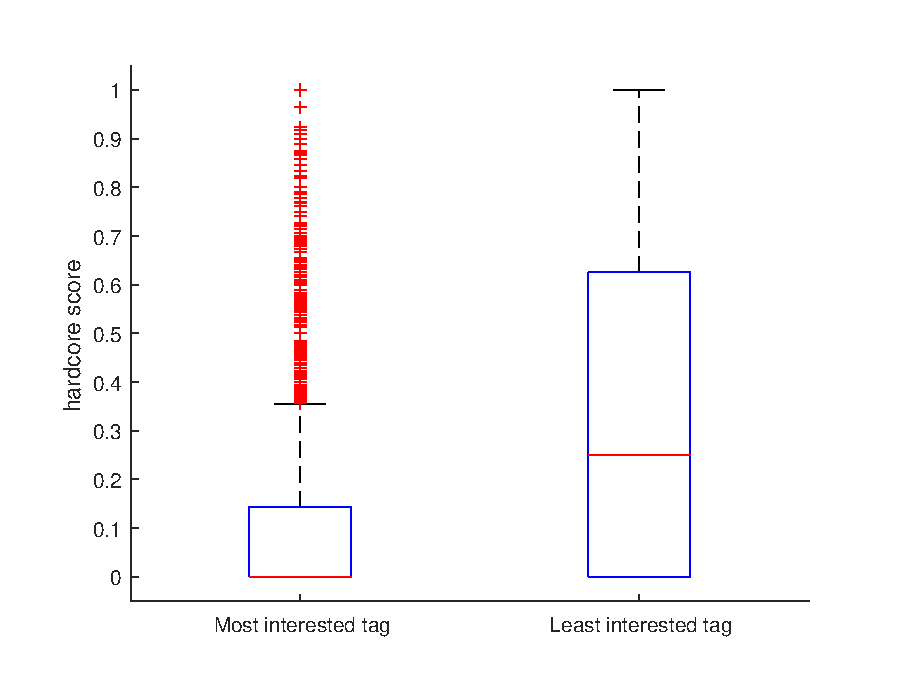
\includegraphics[width=0.2\textwidth]{fig10_eachmovie.eps}
}
\caption{The distribution of hardcore scores upon personal interest}
\label{fig:personalinterest}
\end{figure}

Is hardcore related to moral basis? We define two moral situations in Recommender Systems, one is to praise a (wrongly) criticized item, the other is to criticize an (improperly) appreciated item. Following the definition of hardcore score, we compute how people react in giving positive feedback ($r_{i,j}>\hat{r}+\frac{\max{r}-\min{r}}{5}$) to items with average negative feedback ($\hat{r}<3$ in Movielens and Yahoo!, $\hat{r}<0.6$ in Eachmovie) and giving negative feedback ($r_{i,j}<\hat{r}-\frac{\max{r}-\min{r}}{5}$) to items with average positive feedback ($\hat{r}>3$ in Movielens and Yahoo!, $\hat{r}>0.6$ in Eachmovie). As shown in Fig.~\ref{fig:moralbasis}, it is clear that people feel more obligated to save a criticized item than to underrate a highly appreciated item.

\begin{figure}[htbp]
\centering
\centering
\subfigure[Movielens]{
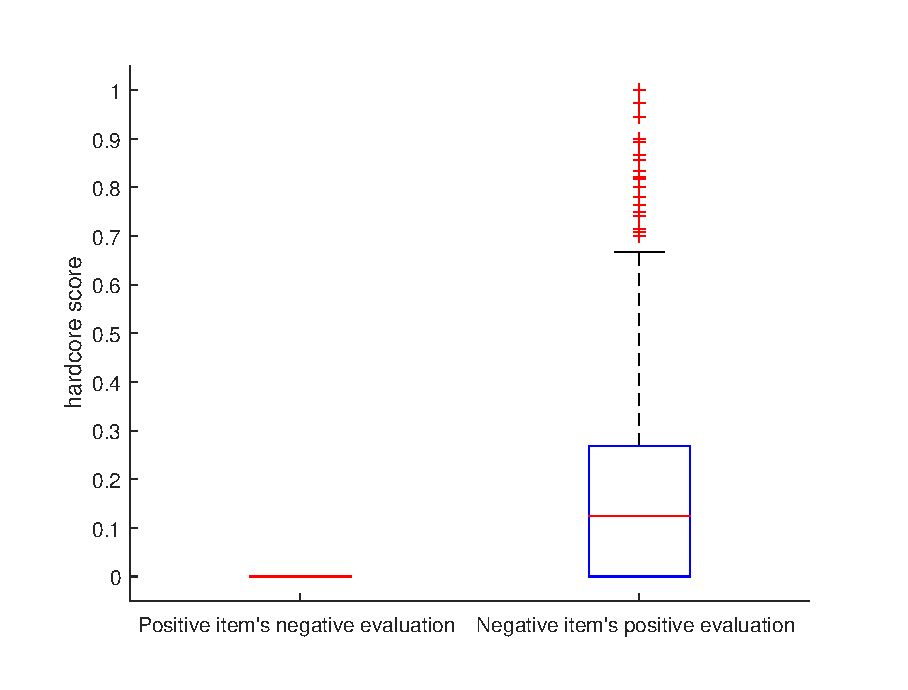
\includegraphics[width=0.2\textwidth]{fig11_movielens1M.eps}
}
\subfigure[Eachmovie]{
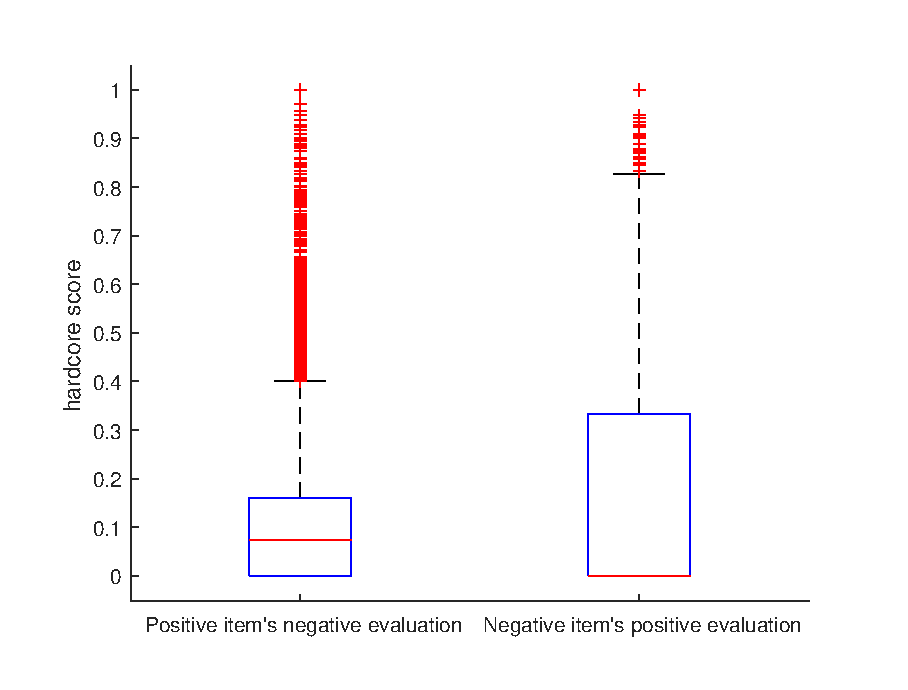
\includegraphics[width=0.2\textwidth]{fig11_eachmovie.eps}
}
\subfigure[Yahoo!random]{
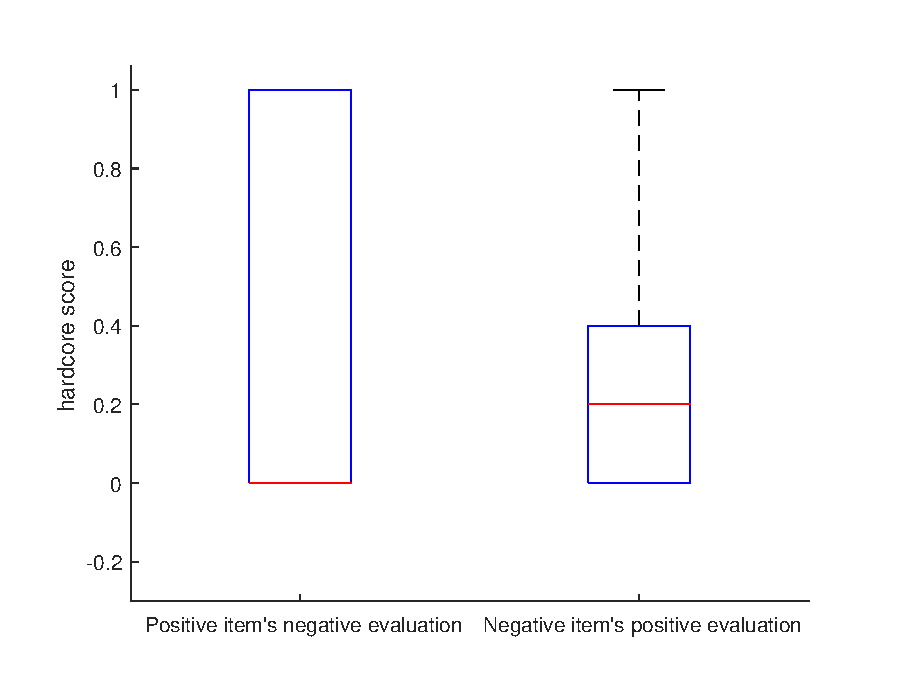
\includegraphics[width=0.2\textwidth]{fig11_random.eps}
}
\subfigure[Yahoo!user]{
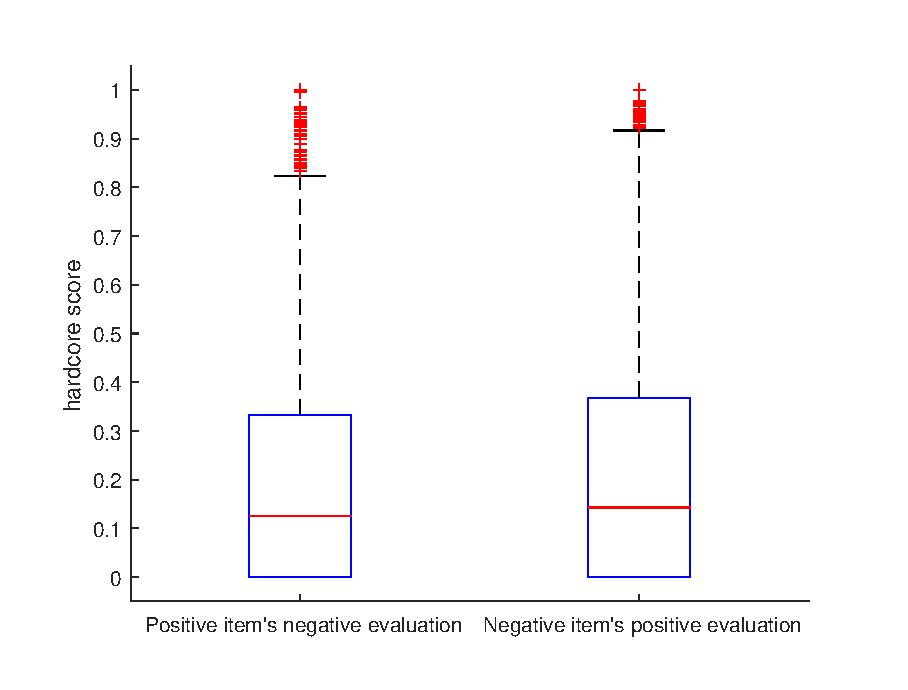
\includegraphics[width=0.2\textwidth]{fig11_user.eps}
}
\caption{The distribution of hardcore scores under two moral situations}
\label{fig:moralbasis}
\end{figure}

We also conduct analysis to correlate hardcore personality to user experience and context of ratings. No evidence is found to imply significant correlation between the probability of a user being hardcore and the number of ratings he/she gives, in which day of a week and which time of a day the rating is given, and the previous items he/she rates. We obmit the analysis here due to the limit of space.

\section{Model}\label{sec:model}

% user : $U_i$, item $V_j$, rating $R$, response $X$




%basic MNAR model
As with most matrix factorization models, we assume there are $K$ hidden aspects. The user preference is denoted as a vector $U_i\in R^K$ , and each item's coefficient to the aspects is denoted as a vector $V_j \in R^K$. We assign a random variable $Bu_i\in R$ to each user and $Bv_j\in R$ to each item to represent the user bias and item bias. The rating given by user $U_i$ to item $V_j$ is denoted by $R_{i,j}$. The ratings are semi-observed. Whether the rating $R_{i,j}$ is observed is denoted by a response variable $X_{i,j}$, where $X_{i,j}=1$ indicates the rating is observed and otherwise the rating is missing. We present four representative models below.

\begin{figure*}[ht]
\centering
\subfigure[Base $\&$ COL]{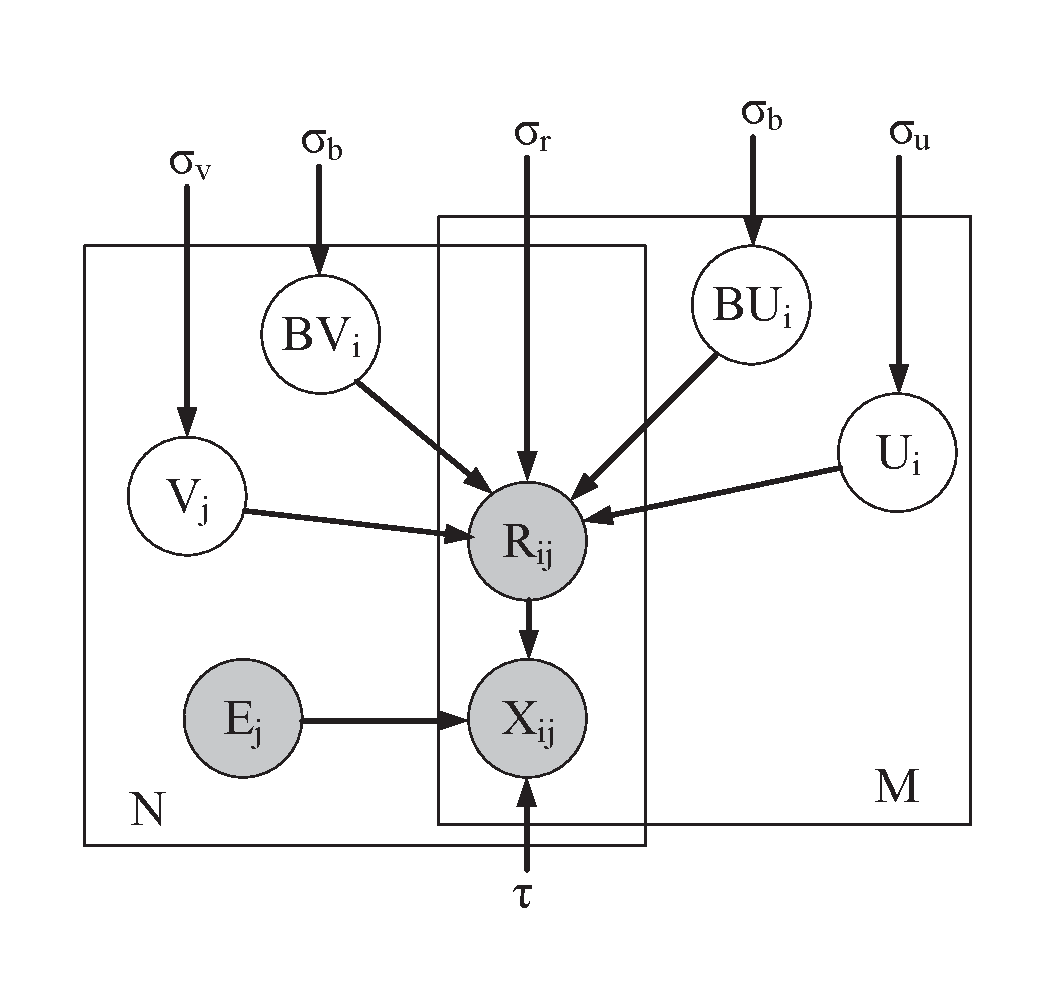
\includegraphics[width=0.35\textwidth]{fig12_Base.eps}\label{fig:basemodel}}
\subfigure[CPC]{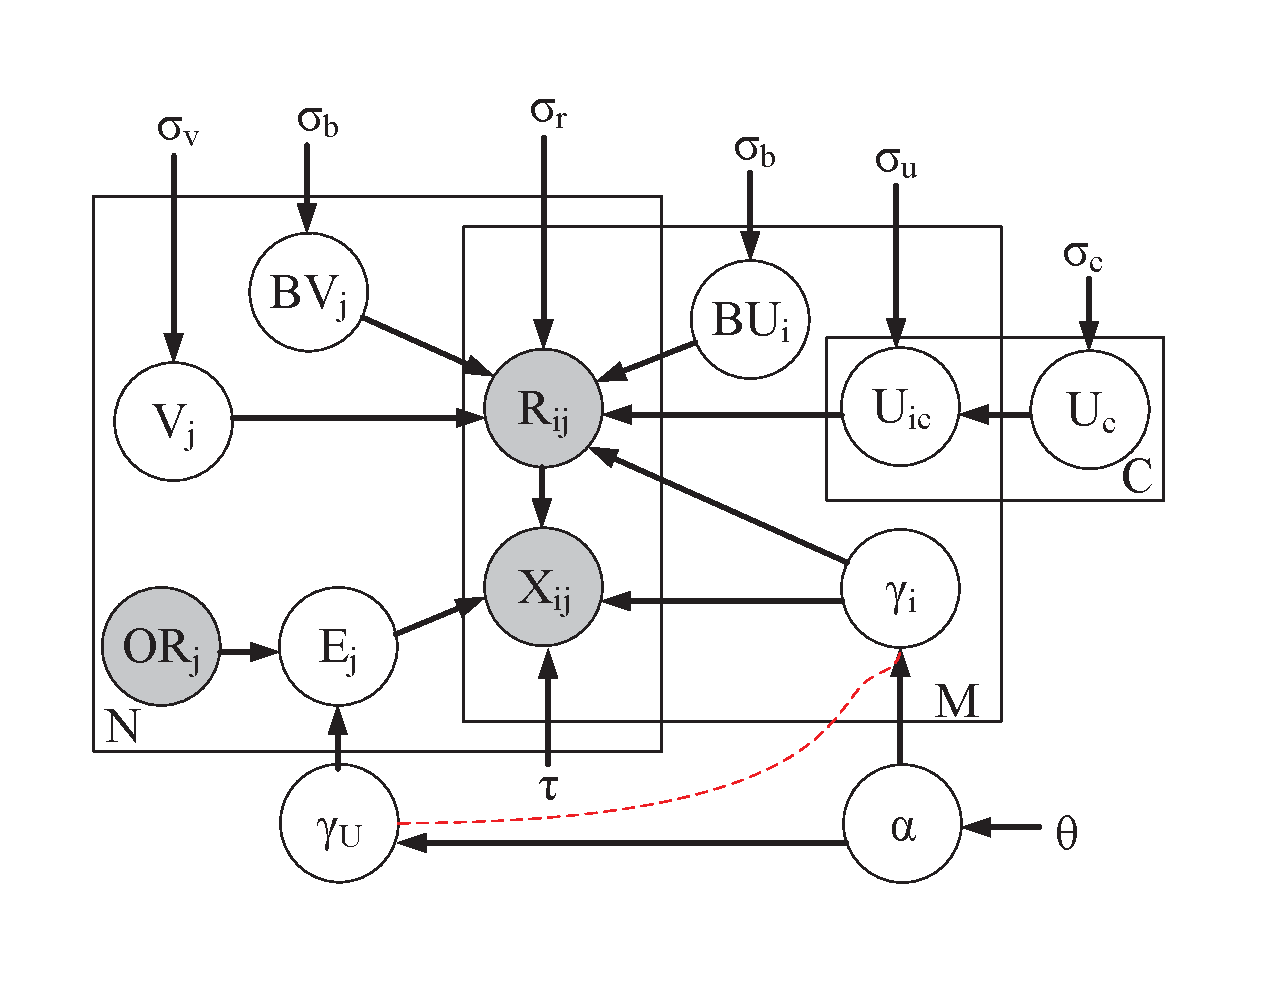
\includegraphics[width=0.4\textwidth]{fig12_CPC.eps}\label{fig:communitymodel}}
\subfigure[CPP]{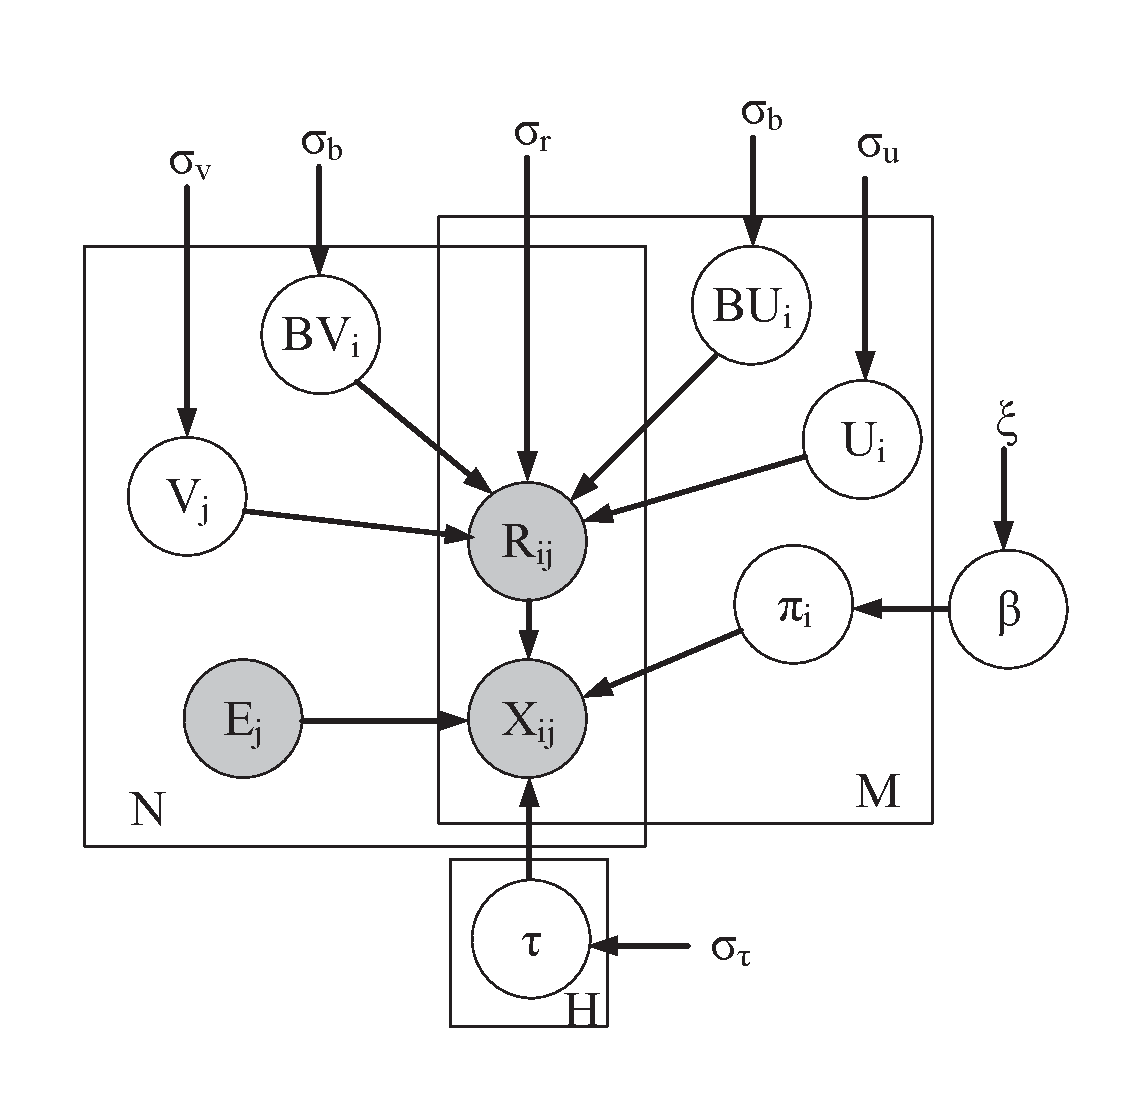
\includegraphics[width=0.4\textwidth]{fig12_CPP.eps}\label{fig:hardcoremodel}}
\subfigure[CPV]{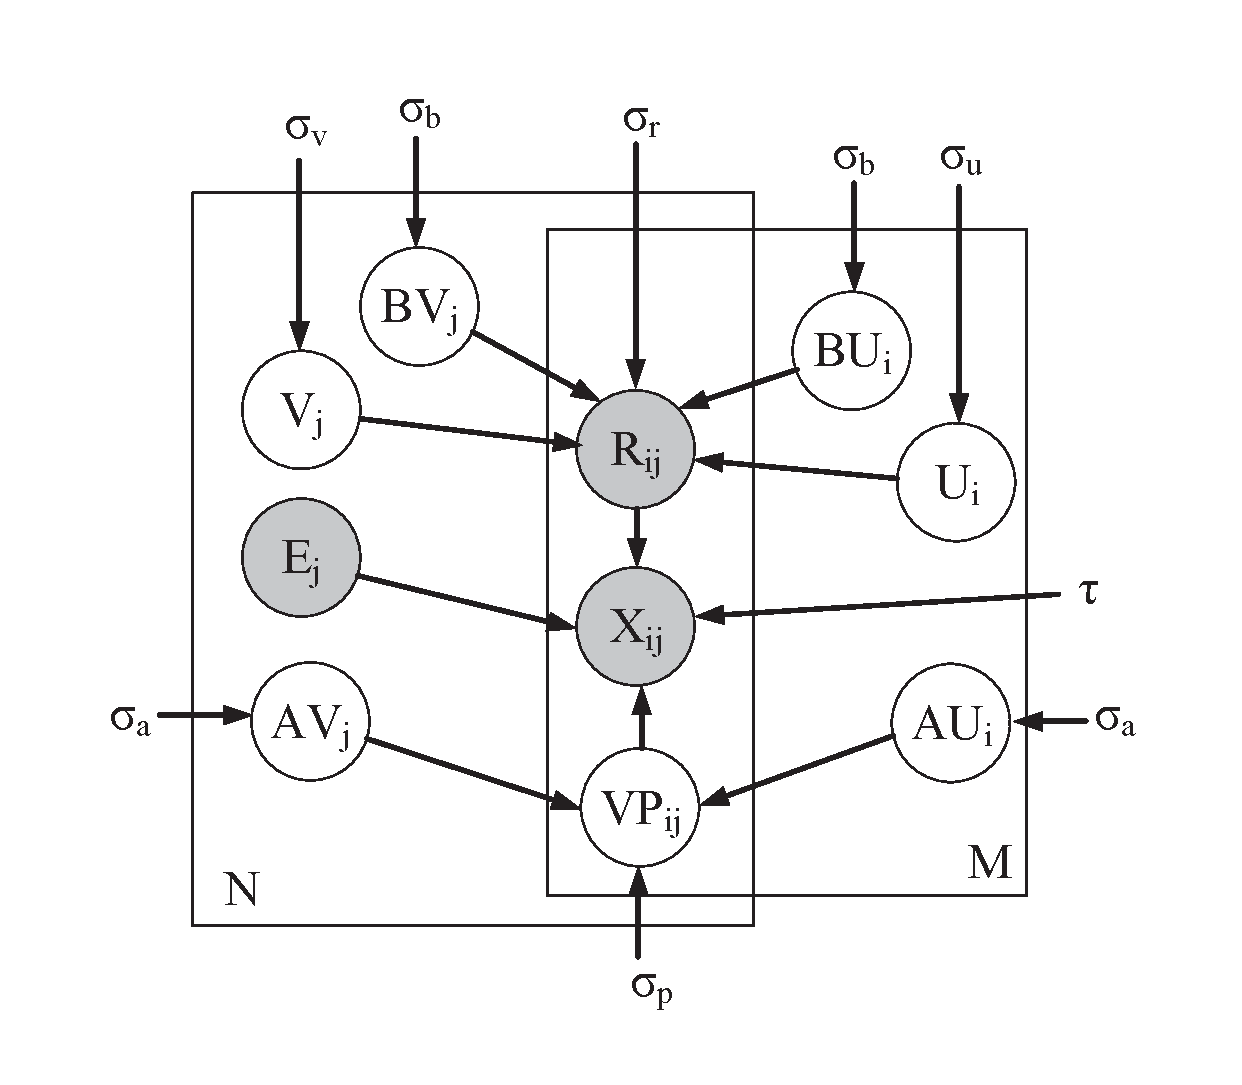
\includegraphics[width=0.4\textwidth]{fig12_CPV.eps}\label{fig:itemmodel}}
\caption{Graphic representation of models}\label{fig:model}
\end{figure*}
\subsection{Model Base and COL}

Intuitively, a user will give a high rating if the item matches his/her preference. If his/her opinion is close to the opinion climate, he/she is more likely to reveal this rating. Furthermore, our  discovery in  empirical study shows that users feel more obligated to give positive feedback on negative items. Taking into account of the above three intuitions, our \textbf{Base} model assumes the following three generative stages.

\textit{The preprocessing stage:} For each user, generate the user preference from a Gaussian distribution with mean $0$.
\begin{equation}\label{equ:preferencebase}
U_i \sim \mathcal{N}(0,\sigma_u^2)
\end{equation}

Similarly, the user bias, item bias and item factors are also generated from Gaussian distributions. $BU_i, BV_j \sim \mathcal{N}(0,\sigma_b^2)$,  $V_j \sim \mathcal{N}(0,\sigma_v^2)$.

\textit{The rating generation stage:} The rating $R_{i,j}=U_iV_j+Bu_i + Bv_j +\epsilon$, where $\epsilon$ is a zero-mean Gaussion error. Hence in this stage, generate the rating: 

\begin{equation}\label{equ:rating}
R_{i,j} \sim \mathcal{N}(U_iV_j+Bu_i+Bv_j, \sigma_r^2)
\end{equation}

\textit{The response generation stage:} Generate the response value $X_{i,j}$ from Equ.\ref{equ:responsebase}

\begin{equation}\label{equ:responsebase}
 P(X_{i,j}=1|R_{i,j},E_j)=\frac{1}{1+\exp{(-\tau(R_{i,j}-E_j))}}
\end{equation}
 where $\tau$ is a strenth parameter, $E_j$ is the opinon climate for the particular item. In the baseline model, we set the opinion climate to be the average of all observed ratings.
\begin{equation}\label{equ:ebase}
 E_j=\frac{\Sigma_jR_{i,j}X_{i,j}}{\Sigma_j X_{i,j}}
\end{equation}


%expert
With a simple modification in the Base model, we obtain the \textbf{Conditional on Opinion Leader (COL)} model. The graphical representation of Base and COL is illustrated in Fig.~\ref{fig:basemodel}. Instead of computing a global majority rating by Equ.\ref{equ:ebase}, the average is taken over some expert users $e$.

\begin{equation}\label{eexpert}
E_j = \frac{\Sigma_e R_{e,j}X_{e,j}}{\Sigma_e X_{e,j}}
\end{equation}

where the experts are extracted by some expert identification algorithms. This allows the flexibility of utilizing side information sources, such as cascaded social networks, to recognize opinion leaders. 

\subsection{Model CPC}
%community
In the \textbf{Conditional Probability on Community (CPC)} model, we introduce a random variable $\gamma_i\in \{0,1\}$ to represent the community assignment of each user.

\begin{equation}
\gamma_{i,c}=
\begin{cases}
1& \text{if user $i$ is in community $c$}\\
0& \text{else}
\end{cases}
\end{equation}

where $\Sigma_c \gamma_{i,c}=1$.  Intuitively, users in the same community share similar preferences. We assume that the ``common'' preference in community $c$, denoted by $U_c$ is generated from a zero-mean Gaussian distribution $U_c \sim \mathcal{N}(0,\sigma_u^2)$. Thus as summarized in Fig.~\ref{fig:communitymodel}, the \textit{preprocessing stage} is as follows.

Generate a global community distribution $\alpha\sim Dir(\theta), \Sigma_c \alpha_c=1, \forall \alpha_c>0$. For each user, first generate the community indicator $\gamma_i \sim Discrete(\alpha)$, then generate the user preference according to his/her community:

\begin{equation}\label{equ:preferencebase}
U_i \sim \Pi_c \mathcal{N}(U_c,\sigma_u^2)^{\gamma_{i,c}}
\end{equation}

In the \textit{response generation stage}, we replace the opinion climate in Equ.\ref{equ:ebase} by a community specific opinion climate.

\begin{equation}\label{equ:ecommunity}
 E_{c,j}=\frac{\Sigma_j\gamma_{i,c} R_{i,j}X_{i,j}}{\Sigma_j \gamma_{i,c} X_{i,j}}
\end{equation}

\subsection{Model CPP}
%user personality
To model the split of users between hardcore and normal groups, the  \textbf{Conditional Probability on Persona (CPP)} model,  shown in Fig.~\ref{fig:hardcoremodel}, introduces a  persona variable,  denoted by $\pi \in \{0,1\}$. Intuitively, when a user is hardcore $\pi_{i,0}=1$ indicates that the user is more likely to speak out regardless of the opinion climate. Thus the strength parameter $\tau$ is reasonably smaller.  

In the \textit{preprocessing stage}, draw a persona distribution from a Beta distribution $\beta \sim \mathcal{B}(\xi), 0<\beta<1$. For each persona, Draw a hardcore coefficient $\tau_z \sim \mathcal{N}(1,\sigma_\tau), z\in \{0,1\}$. For each user, draw a persona from a Bernouli distribution $\pi_i \sim Bern (\beta)$. 

In the \textit{response generation stage}, generate the response value $X_{i,j}$ from Equ.\ref{equ:responseCPP}

\begin{equation}\label{equ:responseCPP}
 P(X_{i,j}=1|R_{i,j},E_j)=\Pi_z {\frac{1}{1+\exp{(-\tau_z(R_{i,j}-E_j))}}}^{\pi_{i,z}}
\end{equation}

\subsection{Model CPV}
%item popularity
Finally we give model \textbf{CPV} to associate the silence strategy to the nature of items. As shown in Fig.~\ref{fig:itemmodel}, we introduce auxilary variable $AU_i\in R^K$ to represent user activity, $AV_j\in R^K$ to represent item attention potential, $Vp_j$ to represent item popularity. Intuitively, if a user is more active, then he/she is able to witness more items. If an item has the potential to become a best seller, then it will receive more attentions. In the \textit{preprocessing stage}, we have  $AU_i, AV_j \sim \mathcal{N}(0,\sigma_a^2)$


In the \textit{rating generation stage}, in addition to Eq.~\ref{equ:rating}, we generate an item popularity score.

\begin{equation}\label{equ:popularity}
VP_j\sim \mathcal{N}(AU_i AV_j,\sigma_p^2) 
\end{equation} 

Consequently, we modified the response probability to

\begin{equation}\label{equ:responseCPV}
P(x_{i,j}|r_{i,j},E_{c,j},\gamma)=\frac{1}{1+\exp{(-\tau(r_{i,j}-E_{c,j}-VP_j))}}
\end{equation}



\subsection{Inference}

We apply EM algorithms to infer the model parameters. In model Base and COL, the update equations are
\begin{eqnarray}
U_i \leftarrow & \\\nonumber
V_j \leftarrow & \\\nonumber
\end{eqnarray}

In model CPC, the log-likelihood is  
\begin{equation*}
\begin{split}
\mathcal{L}_{CPC}=&\sum\limits_{i=1}^{M}\sum\limits_{c=1}^{C}\gamma_{i,c}(log(\alpha_c)+\sum\limits_{j=1}^{N}log(\omega_{i,j,c}))\\\nonumber
&+log(D(\alpha|\theta))+log(\mathcal{N}(U_c|0, \sigma^2_c))\\\nonumber
&+log(\mathcal{N}(U_{i,c}|U_c, \sigma^2_u))+log(\mathcal{N}(V_j|0,\sigma^2_v))\\\nonumber
&+log(\mathcal{N}(Bu_i|0,\sigma^2_b))+log(\mathcal{N}(Bv_j|0,\sigma^2_b))\\\nonumber
\omega_{i,j,c}=&
\begin{cases}
P(X_{i,j}=1|R_{i,j},E_{c,j})P(R_{i,j})& \text{$X_{i,j}=1$}\\\nonumber
1-P(X_{i,j}=1|R_{i,j},E_{c,j})& \text{$X_{i,j}=0$}
\end{cases}
\end{split}
\end{equation*}

The update equations are
\begin{eqnarray}
U_i \leftarrow & \\\nonumber
V_j \leftarrow &\\\nonumber
\end{eqnarray}


In model CPC, the update equations are:

\begin{eqnarray}
BUP_{i,j,c}\leftarrow & \frac{\tau}{1+e^{(-\tau((r_{i,j}^{[x_{i,j}=1]}p_{i,j,c}^{[x_{i,j}=0]})-m_{j,c}-up_i))}}\\\nonumber
up_i\leftarrow &up_i+lr(\sum\limits_{c=1}^{C}\hat{\gamma_{i,c}}\sum\limits_{j=1}^{N}B_{i,j,c}-up_i)\\\nonumber
BVP_{i,j,c}\leftarrow &\frac{\tau}{1+e^{(-\tau((r_{i,j}^{[x_{i,j}=1]}p_{i,j,c}^{[x_{i,j}=0]})-m_{j,c}-vp_j))}}\\\nonumber
\end{eqnarray}

In model CPV, the update equations:

\begin{eqnarray}
vp_j\leftarrow & vp_j+lr(\sum\limits_{c=1}^{C}\sum\limits_{i=1}^{M}\hat{\gamma_{i,c}}B_{i,j,c}-vp_j)\\\nonumber
\end{eqnarray}


\section{Experiment}\label{sec:experiment}

The data sets used in this section include Yahoo!, movieLen-1M, and eachmovie mentioned above. In addition, we use the Mtweet benchmark with $106,337$ ratings by $3,972$ users on $2,043$ movies crawled from Social Network. In each data sets, we remove users whose number of ratings is less than 10, and items which have less than 10 ratings. For each user, we randomly select 5 ratings to construct the test data sets. All ratings are normalized to the range of $(0,1)$.


\subsection{Comparative Study}

The major evaluation metric is $NDCG@L$, which is a standard measure for ranking systems, and has been used as the primary criteria in many MNAR researches~\cite{Hernandez-Lobato2014Probabilistic,Marlin2009Collaborative}  NDCG@L is short for the normalized discounted cumulative gain for top $L$ results. 
\begin{equation}
NDCG@L=\sum\limits_{i=1}^{M}\frac{\sum_{l=1}^{L}(2^{r_{n}(p(l,n))}-1)/log(1+l)}{M\sum_{l=1}^{L}(2^{r_{n}(t(l,n))}-1)/log(1+l)}
\end{equation}
where $p(l,n)$ is the index of the test items sorted in descending order by predicted ratings, $t(l,n)$ is the index of the test items sorted in descending order by true ratings.

In all our models, we set the aspect numbers $K=5$, community numbers $C=$, hyper-parameters  $\tau=1$ for model Base,COL,CPC and CPV.  $\xi=\theta=2$, All the variances are set to $\sigma_b=\sigma_a=\sigma_r=\sigma_u=\sigma_v=\sigma_\tau=1$. The learning rate is set 0.0001 in Yahoo!, Mtweet and movieLen-1M, 0.001 in Eachmovie. Convergence is obtained when the change in mean log-likelihood $\Delta\bar{L}<0.0001$ or stopped at a maximal $1500$ rounds.


We compare our models to a wide range of available models, including conventional memory-based and model-based collaborative filtering recommenders, MNAR models, and ranking based models. The comparative models include (1)uKNN: the user based K-Nearest Neighbor collaborative filtering recommender; (2) MF: the standard matrix factorization model~\cite{Koren2009Matrix}; (3)PMF: the probabilistic matrix factorization model~\cite{salakhutdinov2008probabilistic}; (4)BPR: a classic ranking based model~\cite{Rendle2009Bayesian} (4)CPT-v and Logit-vd: the first MNAR models~\cite{Marlin2009Collaborative} with $K=10$; (5) MF-MNAR~\cite{Hernandez-Lobato2014Probabilistic}: the probabilistic MNAR model which masks the rating matrix by a response matrix, we set $K=20$; (6)RAPMF~\cite{Yang2015Boosting}: an MNAR model which incorporates users' response models into the probabilistic matrix factorization (parameter $K=5$). The variances for the above models are tuned by cross validation.

As shown in Fig.~\ref{fig:modelNDCG} and Fig.~\ref{fig:compNDCG}, we can see that (1) The four variants of our model outperform all non ranking-based models in terms of NDCG at different lengths, which demonstrates the dominant advantages of adjusting a opinion climate in the MNAR models.  (2) CPC performs consistently best in all NDCGs, which is corresponding to our discovery that the user perceiveness of opinion climate is affected by the community. (3) COL, CPP and CPV are better than the base model, which verifies our empirical findings. (4) BPR is the second best in all NDCGs, as BPR directly optimizes the ranking of items.   


\begin{figure*}[!htbp]
\centering
\subfigure[Our models]{
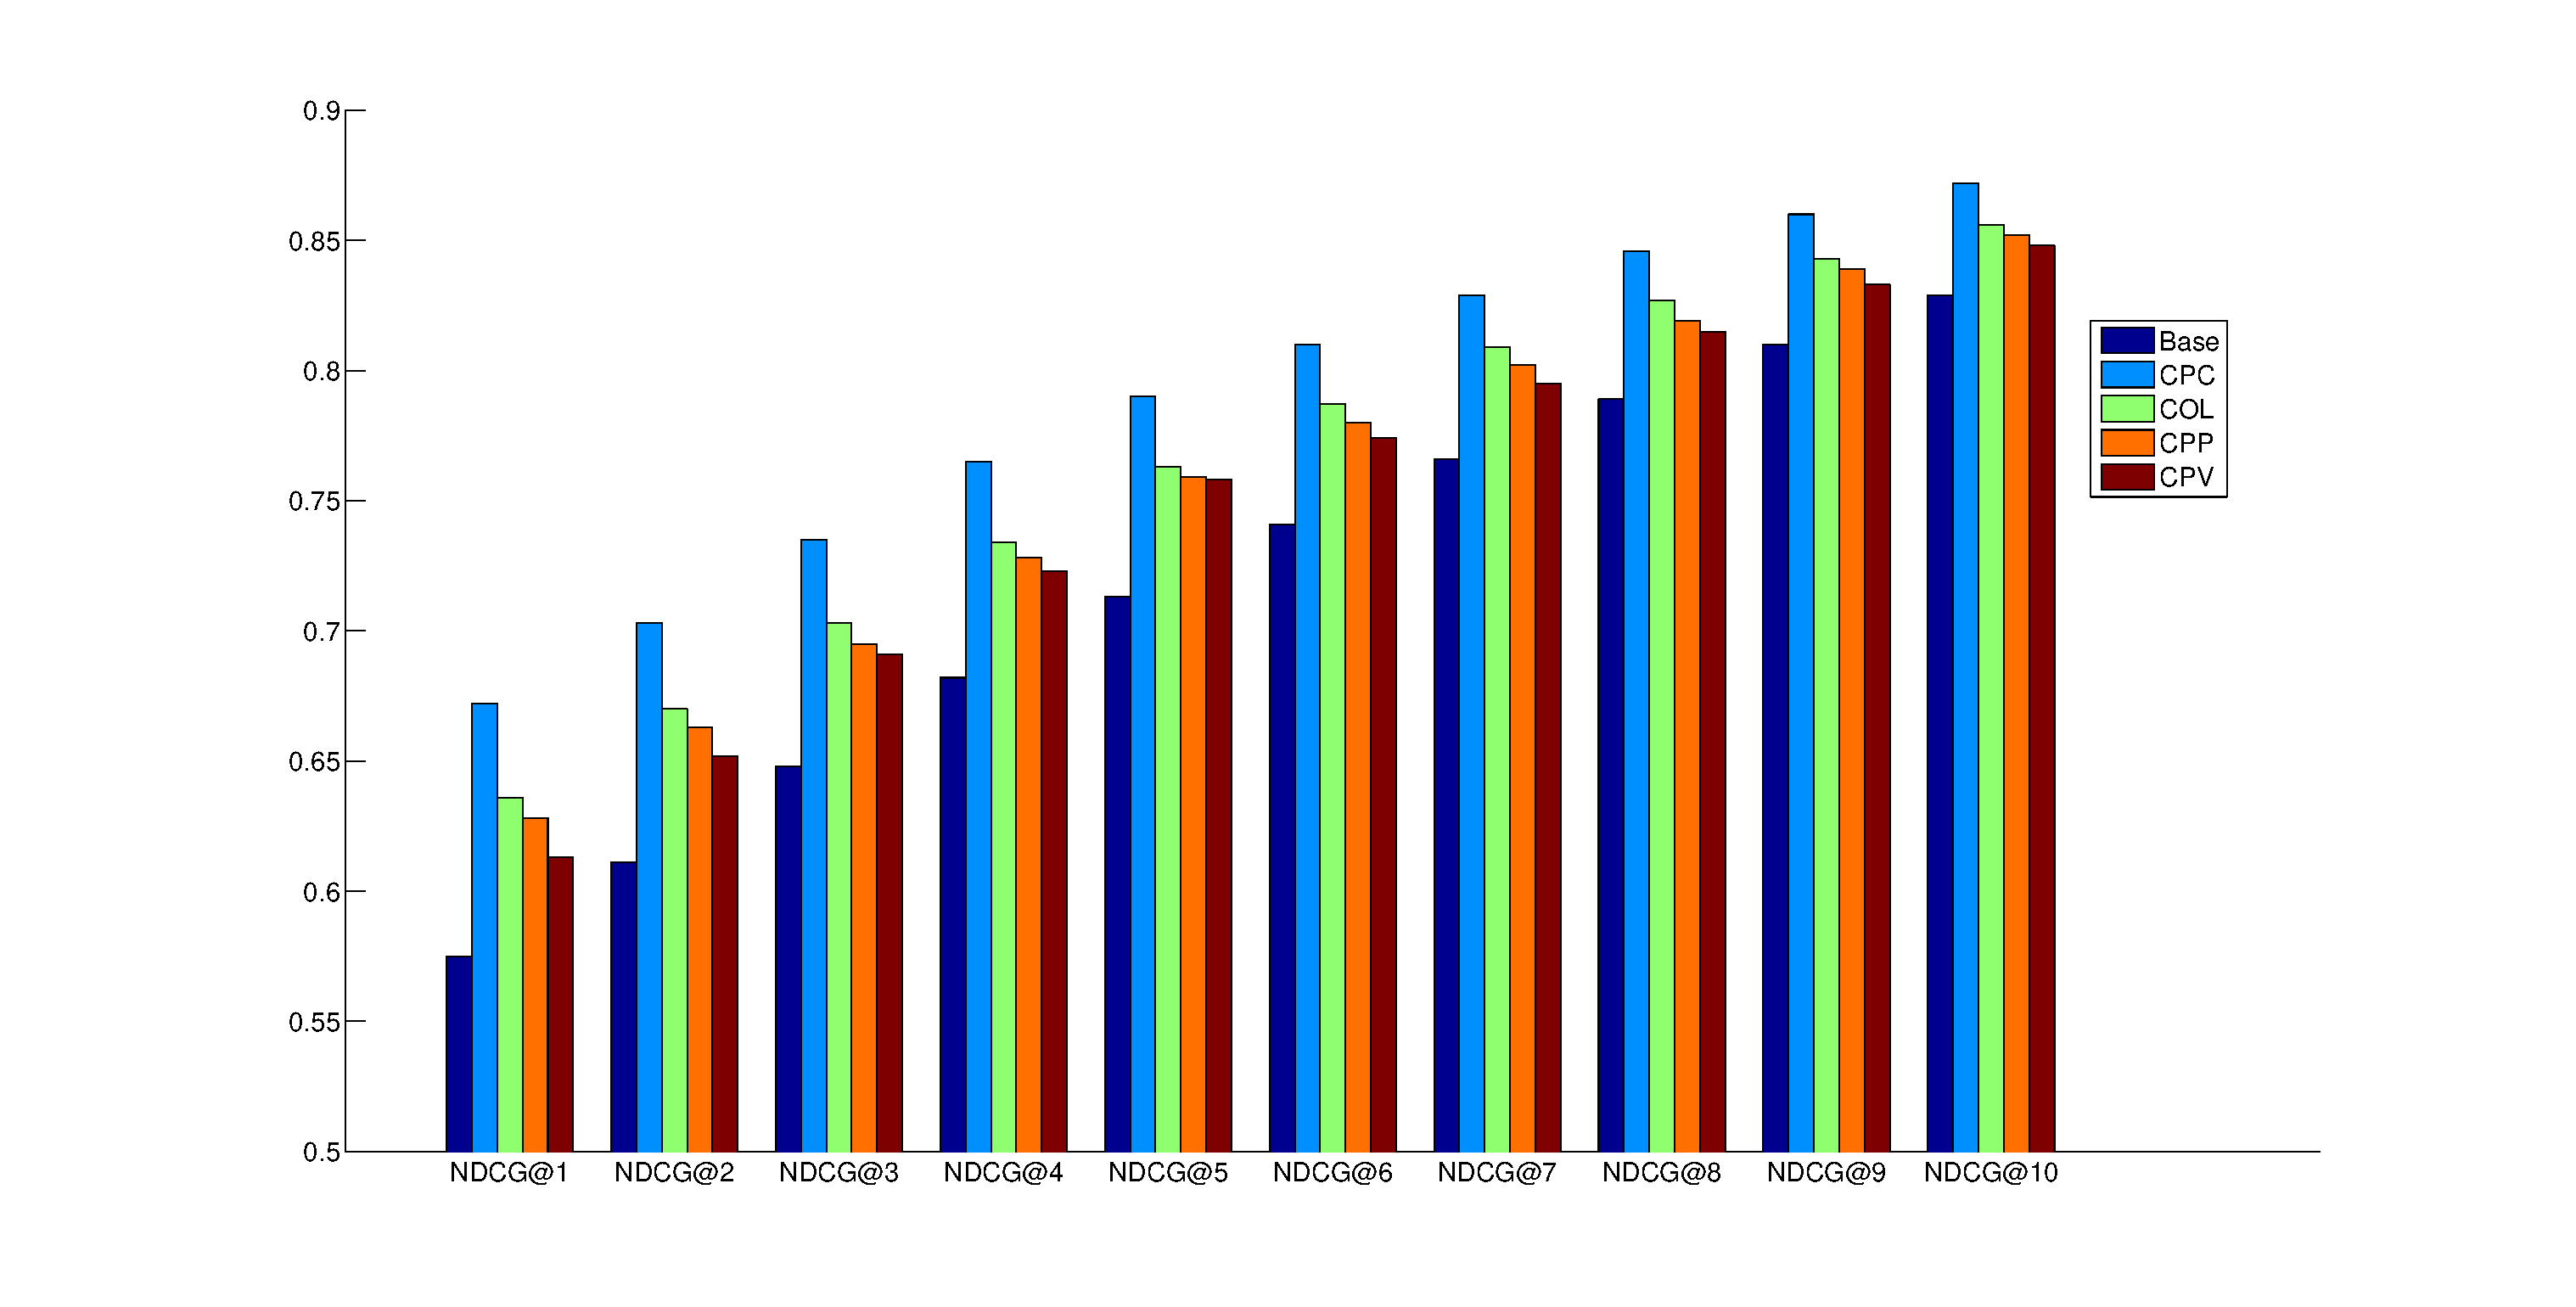
\includegraphics[width=0.9\textwidth]{fig13_model_NDCG.eps}\label{fig:modelNDCG}}
\subfigure[CPC v.s. state-of-the-art models]{
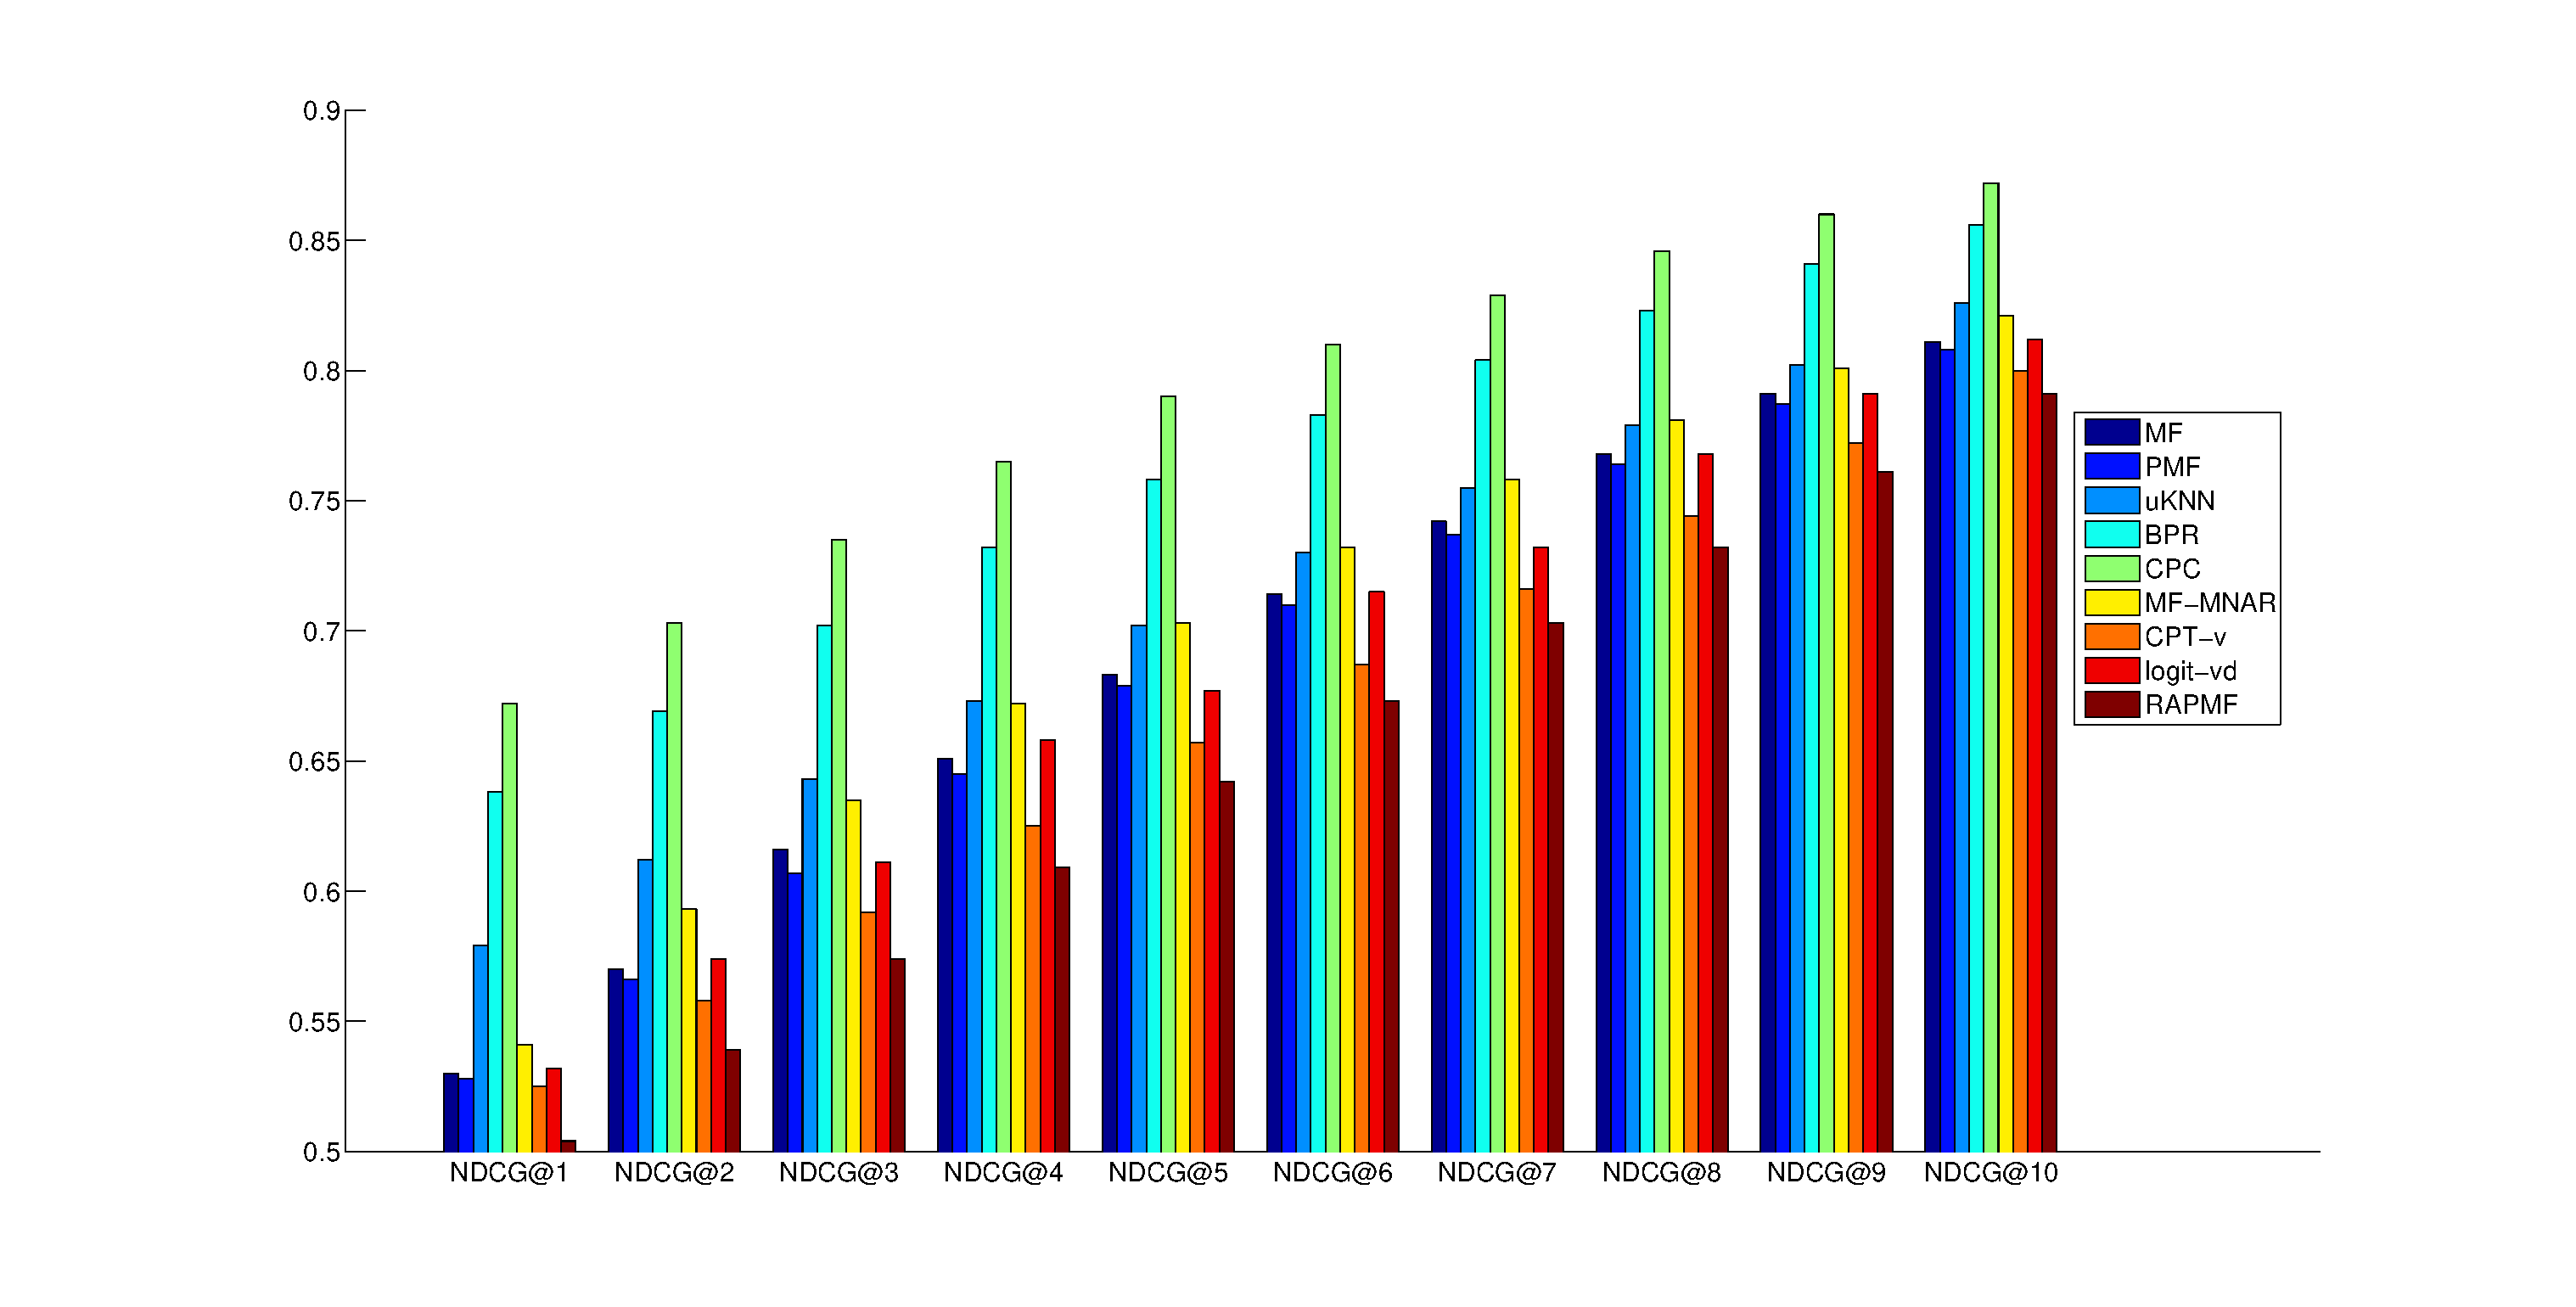
\includegraphics[width=0.9\textwidth]{fig13_compare_NDCG.eps}}\label{fig:compNDCG}
\caption{comparable experiment NDCG performance at top L items}
\end{figure*}


\subsection{Parameter Tunning}
We have two important parameters in our models $\tau$ and $K$. In order to see the effects of these parameters, we set $\tau=0.5,1,1.5,2$ and $K=5,10,15,20$. The $NDCG@5$ result is shown in Fig.~\ref{fig:parameter}. We can conclude that (1) the performance is quite stable, no matter how we set the parameters. (2) The best result is achieved when $\tau=1.5,K=10$. It suggests that the hardcore effect is relative strong as $\tau>1$.
\begin{figure}[htbp]
\centering
\subfigure[$\tau$]{
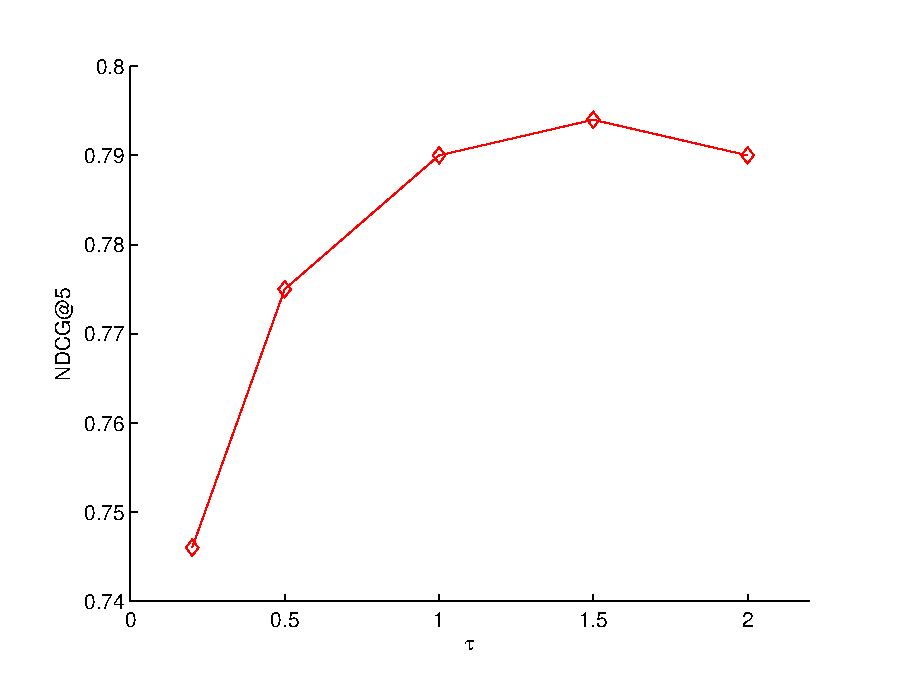
\includegraphics[width=0.2\textwidth]{fig14_tau.eps}}
\subfigure[$K$]{
\includegraphics[width=0.2\textwidth]{fig14_K.eps}}
\caption{NDCG@5 performance over different values of parameters}\label{fig:parameter}
\end{figure}

\subsection{AUC Performance}
Finally, we provide a supplementary experiment on the AUC performance. AUC is the area under recall-precision curve, which is a common measure to evaluate the performance of a binary classifier. We should note that AUC does not reflect how the RS captures MNAR ratings. Therfore, AUC is not the primary measurement for MNAR models. However, as shown in Tab.~\ref{tab:AUC}, our models achive best results in two data sets (Yahoo! and Mtweet) and second best results in the remaining two data sets (Movielens and Eachmovie). Thus our models are comparable to the state-of-the art models in term of AUC evaluation. Furthermore, we observe that CPC and COL are comparable when evaluated by AUC.   

\begin{table*}[htbp]
\centering
\caption{Comparative AUC Performances}\label{tab:AUC}
\centering
\begin{tabular}{|c|c|c|c|c|c|c|c|c|c|c|c|}
\hline
& Base & CPC & COL & CPP & CPV & uKNN & PMF & CPT-v & logit-vd & MF-MNAR & RAPMF \\\hline
\hline
Yahoo & $0.803$ & $0.880$ & $\bf{0.882}$ & $0.857$ & $0.345$ & $0.776$ & $0.504$ & $0.825$ & $0.841$ & $0.863$ & $0.535$ \\\hline
Mtweet & $0.823$ & $\bf{0.864}$ & $\bf{0.863}$ & $0.832$ & $0.823$ & $0.766$ & $0.556$ & $0.828$ & $0.832$ & $0.856$ & $0.582$ \\\hline
MovieLen & $0.874$ & $0.898$ & $\bf{0.902}$ & $0.871$ & $0.517$ & $0.818$ & $0.705$ & $0.878$ & $0.882$ & $\bf{0.929}$ & $0.662$ \\\hline
Eachmovie & $0.840$ & $\bf{0.905}$ & $0.900$ & $0.864$ & $0.776$ & $0.739$ & $0.603$ & $0.792$ & $0.821$ & $\bf{0.912}$ & $0.562$ \\\hline
\end{tabular}
\end{table*}

\section{Conclusion}\label{sec:conclusion}

In this contribution we verify the ``spiral of silence'' theory in real recommender systems. We use the empirical discovies to build recommender models that outperform state-of-the-art recommenders. In the future, we plan to investigate how the empirical discoveries can be combined to improve performances.


\balancecolumns
%\bibliographystyle{abbrv}
%\bibliography{D:/MyRef/MyRef/Reference}

\begin{thebibliography}{10}

\bibitem{Carroll1997Perceived}
J.~G. Carroll, F.~H. Andrew, and J.~Shanahan.
\newblock Perceived support for one's opinions and willingness to speak out: A
  meta-analysis of survey studies on the "spiral of silence".
\newblock {\em The Public Opinion Quarterly}, 61(3):452--463, 1997.

\bibitem{Cohen1970dissonance}
J.~B. Cohen and M.~E. Goldberg.
\newblock The dissonance model in post-decision product evaluation.
\newblock {\em Journal of Marketing Research}, pages 315--321, 1970.

\bibitem{Dalvi2013Para}
N.~N. Dalvi, R.~Kumar, and B.~Pang.
\newblock Para 'normal' activity: On the distribution of average ratings.
\newblock In {\em (ICWSM)}, pages 110--119, 2013.

\bibitem{Godes2012Sequential}
D.~Godes and J.~C. Silva.
\newblock Sequential and temporal dynamics of online opinion.
\newblock {\em Marketing Science}, 31(3):448--473, 2012.

\bibitem{Gopalan2015Scalable}
P.~Gopalan, J.~Hofman, and D.~Blei.
\newblock Scalable recommendation with hierarchical poisson factorization.
\newblock In {\em UAI},
  2015.

\bibitem{Hernandez-Lobato2014Probabilistic}
J.~M. Hernandez-Lobato, N.~Houlsby, and Z.~Ghahramani.
\newblock Probabilistic matrix factorization with non-random missing data.
\newblock In {\em ICML}, 2014.

\bibitem{Hu2009Overcoming}
N.~Hu, J.~Zhang, and P.~A. Pavlou.
\newblock Overcoming the j-shaped distribution of product reviews.
\newblock {\em Commun. ACM}, 52(10):144--147, Oct. 2009.

\bibitem{Jamali2011Generalized}
M.~Jamali, T.~Huang, and M.~Ester.
\newblock A generalized stochastic block model for recommendation in social
  rating networks.
\newblock In {\em RecSys } 2011, pages 53--60.

\bibitem{Jindal2008Opinion}
N.~Jindal and B.~Liu.
\newblock Opinion spam and analysis.
\newblock In {\em  WSDM} 2008, pages 219--230.

\bibitem{Kennamer1990Self}
J.~D. Kennamer.
\newblock Self-serving bibias in perceiving the opinions of others.
\newblock {\em Communication Research}, 17:393--404, 1990.

\bibitem{Kim2014Bayesian}
Y.-D. Kim and S.~Choi.
\newblock Bayesian binomial mixture model for collaborative prediction with
  non-random missing data.
\newblock In {\em  RecSys } 2014, pages 201--208.

\bibitem{Koren2009Matrix}
Y.~Koren, R.~Bell, and C.~Volinsky.
\newblock Matrix factorization techniques for recommender systems.
\newblock {\em Computer}, 42(8):30--37, 2009.

\bibitem{Liang2016Modeling}
D.~Liang, L.~Charlin, J.~McInerney, and D.~M. Blei.
\newblock Modeling user exposure in recommendation.
\newblock In {\em WWW } 2016, pages 951--961.

\bibitem{Ling2012Response}
G.~Ling, H.~Yang, M.~R. Lyu, and I.~King.
\newblock Response aware model-based collaborative filtering.
\newblock In {\em UAI}, pages 501--510, 2012.

\bibitem{Liu2011Wisdom}
N.~N. Liu, X.~Meng, C.~Liu, and Q.~Yang.
\newblock Wisdom of the better few: Cold start recommendation via
  representative based rating elicitation.
\newblock In {\em  RecSys } 2011, pages 37--44.

\bibitem{Marlin2009Collaborative}
B.~M. Marlin and R.~S. Zemel.
\newblock Collaborative prediction and ranking with non-random missing data.
\newblock In {\em RecSys}  2009, pages 5--12.

\bibitem{mcdevitt2003spiral}
M.~McDevitt, S.~Kiousis, and K.~Wahl-Jorgensen.
\newblock Spiral of moderation: Opinion expression in computer-mediated
  discussion.
\newblock {\em International Journal of Public Opinion Research},
  15(4):454--470, 2003.

\bibitem{Neolle-Neumann1993spiral}
E.~Neolle-Neumann.
\newblock {\em The spiral of silence: Public opinion, our social skin.}
\newblock University of Chicago Press., 1993.

\bibitem{Ohsawa2016Gated}
S.~Ohsawa, Y.~Obara, and T.~Osogami.
\newblock Gated probabilistic matrix factorization: Learning users鈥?attention
  from missing values.
\newblock In {\em IJCAI}, pages 1888--1894, 2016.

\bibitem{Pradel2012Ranking}
B.~Pradel, N.~Usunier, and P.~Gallinari.
\newblock Ranking with non-random missing ratings: Influence of popularity and
  positivity on evaluation metrics.
\newblock In {\em RecSys } 2012, pages 147--154.

\bibitem{salakhutdinov2008probabilistic}
R.~Salakhutdinov and A.~Mnih.
\newblock Probabilistic matrix factorization.
\newblock {\em NIPS},
  20:1257--1264, 2008.

\bibitem{Steck2010Training}
H.~Steck.
\newblock Training and testing of recommender systems on data missing not at
  random.
\newblock In {\em SIGKDD } 2010, pages 713--722.

\bibitem{Yang2015Boosting}
H.~Yang, G.~Ling, Y.~Su, M.~R. Lyu, and I.~King.
\newblock Boosting response aware model-based collaborative filtering.
\newblock {\em IEEE Transactions on Knowledge and Data Engineering},
  27(8):2064--2077, Aug 2015.

\end{thebibliography}


\end{document}
